
%% bare_jrnl_compsoc.tex
%% V1.3
%% 2007/01/11
%% by Michael Shell
%% See:
%% http://www.michaelshell.org/
%% for current contact information.
%%
%% This is a skeleton file demonstrating the use of IEEEtran.cls
%% (requires IEEEtran.cls version 1.7 or later) with an IEEE Computer
%% Society journal paper.
%%
%% Support sites:
%% http://www.michaelshell.org/tex/ieeetran/
%% http://www.ctan.org/tex-archive/macros/latex/contrib/IEEEtran/
%% and
%% http://www.ieee.org/

%%*************************************************************************
%% Legal Notice:
%% This code is offered as-is without any warranty either expressed or
%% implied; without even the implied warranty of MERCHANTABILITY or
%% FITNESS FOR A PARTICULAR PURPOSE! 
%% User assumes all risk.
%% In no event shall IEEE or any contributor to this code be liable for
%% any damages or losses, including, but not limited to, incidental,
%% consequential, or any other damages, resulting from the use or misuse
%% of any information contained here.
%%
%% All comments are the opinions of their respective authors and are not
%% necessarily endorsed by the IEEE.
%%
%% This work is distributed under the LaTeX Project Public License (LPPL)
%% ( http://www.latex-project.org/ ) version 1.3, and may be freely used,
%% distributed and modified. A copy of the LPPL, version 1.3, is included
%% in the base LaTeX documentation of all distributions of LaTeX released
%% 2003/12/01 or later.
%% Retain all contribution notices and credits.
%% ** Modified files should be clearly indicated as such, including  **
%% ** renaming them and changing author support contact information. **
%%
%% File list of work: IEEEtran.cls, IEEEtran_HOWTO.pdf, bare_adv.tex,
%%                    bare_conf.tex, bare_jrnl.tex, bare_jrnl_compsoc.tex
%%*************************************************************************

% *** Authors should verify (and, if needed, correct) their LaTeX system  ***
% *** with the testflow diagnostic prior to trusting their LaTeX platform ***
% *** with production work. IEEE's font choices can trigger bugs that do  ***
% *** not appear when using other class files.                            ***
% The testflow support page is at:
% http://www.michaelshell.org/tex/testflow/




% Note that the a4paper option is mainly intended so that authors in
% countries using A4 can easily print to A4 and see how their papers will
% look in print - the typesetting of the document will not typically be
% affected with changes in paper size (but the bottom and side margins will).
% Use the testflow package mentioned above to verify correct handling of
% both paper sizes by the user's LaTeX system.
%
% Also note that the "draftcls" or "draftclsnofoot", not "draft", option
% should be used if it is desired that the figures are to be displayed in
% draft mode.
%
% The Computer Society usually requires 10pt for submissions.
%
\documentclass[10pt,journal,cspaper,compsoc]{IEEEtran}
% \usepackage[paper=letterpaper]{geometry} 
\usepackage{natbib}
\usepackage[pdftex]{graphicx}
\usepackage{subfig}
\usepackage{url}
\graphicspath{{images/}}

%
% If IEEEtran.cls has not been installed into the LaTeX system files,
% manually specify the path to it like:
% \documentclass[12pt,journal,compsoc]{../sty/IEEEtran}





% Some very useful LaTeX packages include:
% (uncomment the ones you want to load)


% *** MISC UTILITY PACKAGES ***
%
%\usepackage{ifpdf}
% Heiko Oberdiek's ifpdf.sty is very useful if you need conditional
% compilation based on whether the output is pdf or dvi.
% usage:
% \ifpdf
%   % pdf code
% \else
%   % dvi code
% \fi
% The latest version of ifpdf.sty can be obtained from:
% http://www.ctan.org/tex-archive/macros/latex/contrib/oberdiek/
% Also, note that IEEEtran.cls V1.7 and later provides a builtin
% \ifCLASSINFOpdf conditional that works the same way.
% When switching from latex to pdflatex and vice-versa, the compiler may
% have to be run twice to clear warning/error messages.






% *** CITATION PACKAGES ***
%
\ifCLASSOPTIONcompsoc
  % IEEE Computer Society needs nocompress option
  % requires cite.sty v4.0 or later (November 2003)
  % \usepackage[nocompress]{cite}
\else
  % normal IEEE
  % \usepackage{cite}
\fi
% cite.sty was written by Donald Arseneau
% V1.6 and later of IEEEtran pre-defines the format of the cite.sty package
% \cite{} output to follow that of IEEE. Loading the cite package will
% result in citation numbers being automatically sorted and properly
% "compressed/ranged". e.g., [1], [9], [2], [7], [5], [6] without using
% cite.sty will become [1], [2], [5]--[7], [9] using cite.sty. cite.sty's
% \cite will automatically add leading space, if needed. Use cite.sty's
% noadjust option (cite.sty V3.8 and later) if you want to turn this off.
% cite.sty is already installed on most LaTeX systems. Be sure and use
% version 4.0 (2003-05-27) and later if using hyperref.sty. cite.sty does
% not currently provide for hyperlinked citations.
% The latest version can be obtained at:
% http://www.ctan.org/tex-archive/macros/latex/contrib/cite/
% The documentation is contained in the cite.sty file itself.
%
% Note that some packages require special options to format as the Computer
% Society requires. In particular, Computer Society  papers do not use
% compressed citation ranges as is done in typical IEEE papers
% (e.g., [1]-[4]). Instead, they list every citation separately in order
% (e.g., [1], [2], [3], [4]). To get the latter we need to load the cite
% package with the nocompress option which is supported by cite.sty v4.0
% and later. Note also the use of a CLASSOPTION conditional provided by
% IEEEtran.cls V1.7 and later.





% *** GRAPHICS RELATED PACKAGES ***
%
\ifCLASSINFOpdf
  % \usepackage[pdftex]{graphicx}
  % declare the path(s) where your graphic files are
  % \graphicspath{{../pdf/}{../jpeg/}}
  % and their extensions so you won't have to specify these with
  % every instance of \includegraphics
  % \DeclareGraphicsExtensions{.pdf,.jpeg,.png}
\else
  % or other class option (dvipsone, dvipdf, if not using dvips). graphicx
  % will default to the driver specified in the system graphics.cfg if no
  % driver is specified.
  % \usepackage[dvips]{graphicx}
  % declare the path(s) where your graphic files are
  % \graphicspath{{../eps/}}
  % and their extensions so you won't have to specify these with
  % every instance of \includegraphics
  % \DeclareGraphicsExtensions{.eps}
\fi
% graphicx was written by David Carlisle and Sebastian Rahtz. It is
% required if you want graphics, photos, etc. graphicx.sty is already
% installed on most LaTeX systems. The latest version and documentation can
% be obtained at: 
% http://www.ctan.org/tex-archive/macros/latex/required/graphics/
% Another good source of documentation is "Using Imported Graphics in
% LaTeX2e" by Keith Reckdahl which can be found as epslatex.ps or
% epslatex.pdf at: http://www.ctan.org/tex-archive/info/
%
% latex, and pdflatex in dvi mode, support graphics in encapsulated
% postscript (.eps) format. pdflatex in pdf mode supports graphics
% in .pdf, .jpeg, .png and .mps (metapost) formats. Users should ensure
% that all non-photo figures use a vector format (.eps, .pdf, .mps) and
% not a bitmapped formats (.jpeg, .png). IEEE frowns on bitmapped formats
% which can result in "jaggedy"/blurry rendering of lines and letters as
% well as large increases in file sizes.
%
% You can find documentation about the pdfTeX application at:
% http://www.tug.org/applications/pdftex





% *** MATH PACKAGES ***
%
%\usepackage[cmex10]{amsmath}
% A popular package from the American Mathematical Society that provides
% many useful and powerful commands for dealing with mathematics. If using
% it, be sure to load this package with the cmex10 option to ensure that
% only type 1 fonts will utilized at all point sizes. Without this option,
% it is possible that some math symbols, particularly those within
% footnotes, will be rendered in bitmap form which will result in a
% document that can not be IEEE Xplore compliant!
%
% Also, note that the amsmath package sets \interdisplaylinepenalty to 10000
% thus preventing page breaks from occurring within multiline equations. Use:
%\interdisplaylinepenalty=2500
% after loading amsmath to restore such page breaks as IEEEtran.cls normally
% does. amsmath.sty is already installed on most LaTeX systems. The latest
% version and documentation can be obtained at:
% http://www.ctan.org/tex-archive/macros/latex/required/amslatex/math/





% *** SPECIALIZED LIST PACKAGES ***
%
%\usepackage{algorithmic}
% algorithmic.sty was written by Peter Williams and Rogerio Brito.
% This package provides an algorithmic environment fo describing algorithms.
% You can use the algorithmic environment in-text or within a figure
% environment to provide for a floating algorithm. Do NOT use the algorithm
% floating environment provided by algorithm.sty (by the same authors) or
% algorithm2e.sty (by Christophe Fiorio) as IEEE does not use dedicated
% algorithm float types and packages that provide these will not provide
% correct IEEE style captions. The latest version and documentation of
% algorithmic.sty can be obtained at:
% http://www.ctan.org/tex-archive/macros/latex/contrib/algorithms/
% There is also a support site at:
% http://algorithms.berlios.de/index.html
% Also of interest may be the (relatively newer and more customizable)
% algorithmicx.sty package by Szasz Janos:
% http://www.ctan.org/tex-archive/macros/latex/contrib/algorithmicx/




% *** ALIGNMENT PACKAGES ***
%
%\usepackage{array}
% Frank Mittelbach's and David Carlisle's array.sty patches and improves
% the standard LaTeX2e array and tabular environments to provide better
% appearance and additional user controls. As the default LaTeX2e table
% generation code is lacking to the point of almost being broken with
% respect to the quality of the end results, all users are strongly
% advised to use an enhanced (at the very least that provided by array.sty)
% set of table tools. array.sty is already installed on most systems. The
% latest version and documentation can be obtained at:
% http://www.ctan.org/tex-archive/macros/latex/required/tools/


%\usepackage{mdwmath}
%\usepackage{mdwtab}
% Also highly recommended is Mark Wooding's extremely powerful MDW tools,
% especially mdwmath.sty and mdwtab.sty which are used to format equations
% and tables, respectively. The MDWtools set is already installed on most
% LaTeX systems. The lastest version and documentation is available at:
% http://www.ctan.org/tex-archive/macros/latex/contrib/mdwtools/


% IEEEtran contains the IEEEeqnarray family of commands that can be used to
% generate multiline equations as well as matrices, tables, etc., of high
% quality.


%\usepackage{eqparbox}
% Also of notable interest is Scott Pakin's eqparbox package for creating
% (automatically sized) equal width boxes - aka "natural width parboxes".
% Available at:
% http://www.ctan.org/tex-archive/macros/latex/contrib/eqparbox/





% *** SUBFIGURE PACKAGES ***
%\ifCLASSOPTIONcompsoc
%\usepackage[tight,normalsize,sf,SF]{subfigure}
%\else
%\usepackage[tight,footnotesize]{subfigure}
%\fi
% subfigure.sty was written by Steven Douglas Cochran. This package makes it
% easy to put subfigures in your figures. e.g., "Figure 1a and 1b". For IEEE
% work, it is a good idea to load it with the tight package option to reduce
% the amount of white space around the subfigures. Computer Society papers
% use a larger font and \sffamily font for their captions, hence the
% additional options needed under compsoc mode. subfigure.sty is already
% installed on most LaTeX systems. The latest version and documentation can
% be obtained at:
% http://www.ctan.org/tex-archive/obsolete/macros/latex/contrib/subfigure/
% subfigure.sty has been superceeded by subfig.sty.


%\ifCLASSOPTIONcompsoc
%  \usepackage[caption=false]{caption}
%  \usepackage[font=normalsize,labelfont=sf,textfont=sf]{subfig}
%\else
%  \usepackage[caption=false]{caption}
%  \usepackage[font=footnotesize]{subfig}
%\fi
% subfig.sty, also written by Steven Douglas Cochran, is the modern
% replacement for subfigure.sty. However, subfig.sty requires and
% automatically loads Axel Sommerfeldt's caption.sty which will override
% IEEEtran.cls handling of captions and this will result in nonIEEE style
% figure/table captions. To prevent this problem, be sure and preload
% caption.sty with its "caption=false" package option. This is will preserve
% IEEEtran.cls handing of captions. Version 1.3 (2005/06/28) and later 
% (recommended due to many improvements over 1.2) of subfig.sty supports
% the caption=false option directly:
%\ifCLASSOPTIONcompsoc
%  \usepackage[caption=false,font=normalsize,labelfont=sf,textfont=sf]{subfig}
%\else
%  \usepackage[caption=false,font=footnotesize]{subfig}
%\fi
%
% The latest version and documentation can be obtained at:
% http://www.ctan.org/tex-archive/macros/latex/contrib/subfig/
% The latest version and documentation of caption.sty can be obtained at:
% http://www.ctan.org/tex-archive/macros/latex/contrib/caption/




% *** FLOAT PACKAGES ***
%
%\usepackage{fixltx2e}
% fixltx2e, the successor to the earlier fix2col.sty, was written by
% Frank Mittelbach and David Carlisle. This package corrects a few problems
% in the LaTeX2e kernel, the most notable of which is that in current
% LaTeX2e releases, the ordering of single and double column floats is not
% guaranteed to be preserved. Thus, an unpatched LaTeX2e can allow a
% single column figure to be placed prior to an earlier double column
% figure. The latest version and documentation can be found at:
% http://www.ctan.org/tex-archive/macros/latex/base/



%\usepackage{stfloats}
% stfloats.sty was written by Sigitas Tolusis. This package gives LaTeX2e
% the ability to do double column floats at the bottom of the page as well
% as the top. (e.g., "\begin{figure*}[!b]" is not normally possible in
% LaTeX2e). It also provides a command:
%\fnbelowfloat
% to enable the placement of footnotes below bottom floats (the standard
% LaTeX2e kernel puts them above bottom floats). This is an invasive package
% which rewrites many portions of the LaTeX2e float routines. It may not work
% with other packages that modify the LaTeX2e float routines. The latest
% version and documentation can be obtained at:
% http://www.ctan.org/tex-archive/macros/latex/contrib/sttools/
% Documentation is contained in the stfloats.sty comments as well as in the
% presfull.pdf file. Do not use the stfloats baselinefloat ability as IEEE
% does not allow \baselineskip to stretch. Authors submitting work to the
% IEEE should note that IEEE rarely uses double column equations and
% that authors should try to avoid such use. Do not be tempted to use the
% cuted.sty or midfloat.sty packages (also by Sigitas Tolusis) as IEEE does
% not format its papers in such ways.




%\ifCLASSOPTIONcaptionsoff
%  \usepackage[nomarkers]{endfloat}
% \let\MYoriglatexcaption\caption
% \renewcommand{\caption}[2][\relax]{\MYoriglatexcaption[#2]{#2}}
%\fi
% endfloat.sty was written by James Darrell McCauley and Jeff Goldberg.
% This package may be useful when used in conjunction with IEEEtran.cls'
% captionsoff option. Some IEEE journals/societies require that submissions
% have lists of figures/tables at the end of the paper and that
% figures/tables without any captions are placed on a page by themselves at
% the end of the document. If needed, the draftcls IEEEtran class option or
% \CLASSINPUTbaselinestretch interface can be used to increase the line
% spacing as well. Be sure and use the nomarkers option of endfloat to
% prevent endfloat from "marking" where the figures would have been placed
% in the text. The two hack lines of code above are a slight modification of
% that suggested by in the endfloat docs (section 8.3.1) to ensure that
% the full captions always appear in the list of figures/tables - even if
% the user used the short optional argument of \caption[]{}.
% IEEE papers do not typically make use of \caption[]'s optional argument,
% so this should not be an issue. A similar trick can be used to disable
% captions of packages such as subfig.sty that lack options to turn off
% the subcaptions:
% For subfig.sty:
% \let\MYorigsubfloat\subfloat
% \renewcommand{\subfloat}[2][\relax]{\MYorigsubfloat[]{#2}}
% For subfigure.sty:
% \let\MYorigsubfigure\subfigure
% \renewcommand{\subfigure}[2][\relax]{\MYorigsubfigure[]{#2}}
% However, the above trick will not work if both optional arguments of
% the \subfloat/subfig command are used. Furthermore, there needs to be a
% description of each subfigure *somewhere* and endfloat does not add
% subfigure captions to its list of figures. Thus, the best approach is to
% avoid the use of subfigure captions (many IEEE journals avoid them anyway)
% and instead reference/explain all the subfigures within the main caption.
% The latest version of endfloat.sty and its documentation can obtained at:
% http://www.ctan.org/tex-archive/macros/latex/contrib/endfloat/
%
% The IEEEtran \ifCLASSOPTIONcaptionsoff conditional can also be used
% later in the document, say, to conditionally put the References on a 
% page by themselves.




% *** PDF, URL AND HYPERLINK PACKAGES ***
%
%\usepackage{url}
% url.sty was written by Donald Arseneau. It provides better support for
% handling and breaking URLs. url.sty is already installed on most LaTeX
% systems. The latest version can be obtained at:
% http://www.ctan.org/tex-archive/macros/latex/contrib/misc/
% Read the url.sty source comments for usage information. Basically,
% \url{my_url_here}.





% *** Do not adjust lengths that control margins, column widths, etc. ***
% *** Do not use packages that alter fonts (such as pslatex).         ***
% There should be no need to do such things with IEEEtran.cls V1.6 and later.
% (Unless specifically asked to do so by the journal or conference you plan
% to submit to, of course. )


% correct bad hyphenation here
\hyphenation{op-tical net-works semi-conduc-tor}


\begin{document}
%
% paper title
% can use linebreaks \\ within to get better formatting as desired
\title{Common Angle Charts as perception-true alternative to Parallel Sets}
%
%
% author names and IEEE memberships
% note positions of commas and nonbreaking spaces ( ~ ) LaTeX will not break
% a structure at a ~ so this keeps an author's name from being broken across
% two lines.
% use \thanks{} to gain access to the first footnote area
% a separate \thanks must be used for each paragraph as LaTeX2e's \thanks
% was not built to handle multiple paragraphs
%
%
%\IEEEcompsocitemizethanks is a special \thanks that produces the bulleted
% lists the Computer Society journals use for "first footnote" author
% affiliations. Use \IEEEcompsocthanksitem which works much like \item
% for each affiliation group. When not in compsoc mode,
% \IEEEcompsocitemizethanks becomes like \thanks and
% \IEEEcompsocthanksitem becomes a line break with idention. This
% facilitates dual compilation, although admittedly the differences in the
% desired content of \author between the different types of papers makes a
% one-size-fits-all approach a daunting prospect. For instance, compsoc 
% journal papers have the author affiliations above the "Manuscript
% received ..."  text while in non-compsoc journals this is reversed. Sigh.

\author{Heike~Hofmann,~\IEEEmembership{Member,~IEEE,}
        and~Marie~Vendettuoli% <-this % stops a space
\IEEEcompsocitemizethanks{\IEEEcompsocthanksitem H. Hofmann is faculty member in the Department of Statistics at Iowa State University, IA 50011.\protect\\
% note need leading \protect in front of \\ to get a newline within \thanks as
% \\ is fragile and will error, could use \hfil\break instead.
E-mail: hofmann@iastate.edu
\IEEEcompsocthanksitem M. Vendettuoli is Graduate Student in the HCI and BCB program of Iowa State University and member of working group the USDA in Ames, IA 50014.}% <-this % stops a space
\thanks{}}

% note the % following the last \IEEEmembership and also \thanks - 
% these prevent an unwanted space from occurring between the last author name
% and the end of the author line. i.e., if you had this:
% 
% \author{....lastname \thanks{...} \thanks{...} }
%                     ^------------^------------^----Do not want these spaces!
%
% a space would be appended to the last name and could cause every name on that
% line to be shifted left slightly. This is one of those "LaTeX things". For
% instance, "\textbf{A} \textbf{B}" will typeset as "A B" not "AB". To get
% "AB" then you have to do: "\textbf{A}\textbf{B}"
% \thanks is no different in this regard, so shield the last } of each \thanks
% that ends a line with a % and do not let a space in before the next \thanks.
% Spaces after \IEEEmembership other than the last one are OK (and needed) as
% you are supposed to have spaces between the names. For what it is worth,
% this is a minor point as most people would not even notice if the said evil
% space somehow managed to creep in.



% The paper headers
\markboth{Journal of \LaTeX\ Class Files,~Vol.~6, No.~1, January~2007}%
{Hofmann \MakeLowercase{\textit{et al.}}: Common Angle Plots}
% The only time the second header will appear is for the odd numbered pages
% after the title page when using the twoside option.
% 
% *** Note that you probably will NOT want to include the author's ***
% *** name in the headers of peer review papers.                   ***
% You can use \ifCLASSOPTIONpeerreview for conditional compilation here if
% you desire.



% The publisher's ID mark at the bottom of the page is less important with
% Computer Society journal papers as those publications place the marks
% outside of the main text columns and, therefore, unlike regular IEEE
% journals, the available text space is not reduced by their presence.
% If you want to put a publisher's ID mark on the page you can do it like
% this:
%\IEEEpubid{0000--0000/00\$00.00~\copyright~2007 IEEE}
% or like this to get the Computer Society new two part style.
%\IEEEpubid{\makebox[\columnwidth]{\hfill 0000--0000/00/\$00.00~\copyright~2007 IEEE}%
%\hspace{\columnsep}\makebox[\columnwidth]{Published by the IEEE Computer Society\hfill}}
% Remember, if you use this you must call \IEEEpubidadjcol in the second
% column for its text to clear the IEEEpubid mark (Computer Society jorunal
% papers don't need this extra clearance.)




% for Computer Society papers, we must declare the abstract and index terms
% PRIOR to the title within the \IEEEcompsoctitleabstractindextext IEEEtran
% command as these need to go into the title area created by \maketitle.
\IEEEcompsoctitleabstractindextext{%
\begin{abstract}


\end{abstract}
% IEEEtran.cls defaults to using nonbold math in the Abstract.
% This preserves the distinction between vectors and scalars. However,
% if the journal you are submitting to favors bold math in the abstract,
% then you can use LaTeX's standard command \boldmath at the very start
% of the abstract to achieve this. Many IEEE journals frown on math
% in the abstract anyway. In particular, the Computer Society does
% not want either math or citations to appear in the abstract.

% Note that keywords are not normally used for peer review papers.
\begin{keywords}
Linewidth illusion, Data Visualization, Categorical Variables, Associations
\end{keywords}}


% make the title area
\maketitle


% To allow for easy dual compilation without having to reenter the
% abstract/keywords data, the \IEEEcompsoctitleabstractindextext text will
% not be used in maketitle, but will appear (i.e., to be "transported")
% here as \IEEEdisplaynotcompsoctitleabstractindextext when compsoc mode
% is not selected <OR> if conference mode is selected - because compsoc
% conference papers position the abstract like regular (non-compsoc)
% papers do!
\IEEEdisplaynotcompsoctitleabstractindextext
% \IEEEdisplaynotcompsoctitleabstractindextext has no effect when using
% compsoc under a non-conference mode.


% For peer review papers, you can put extra information on the cover
% page as needed:
% \ifCLASSOPTIONpeerreview
% \begin{center} \bfseries EDICS Category: 3-BBND \end{center}
% \fi
%
% For peerreview papers, this IEEEtran command inserts a page break and
% creates the second title. It will be ignored for other modes.
\IEEEpeerreviewmaketitle



% !TEX root = journal.tex
\section{Introduction}
% Computer Society journal papers do something a tad strange with the very
% first section heading (almost always called "Introduction"). They place it
% ABOVE the main text! IEEEtran.cls currently does not do this for you.
% However, You can achieve this effect by making LaTeX jump through some
% hoops via something like:
%
%\ifCLASSOPTIONcompsoc
%  \noindent\raisebox{2\baselineskip}[0pt][0pt]%
%  {\parbox{\columnwidth}{\section{Introduction}\label{sec:introduction}%
%  \global\everypar=\everypar}}%
%  \vspace{-1\baselineskip}\vspace{-\parskip}\par
%\else
%  \section{Introduction}\label{sec:introduction}\par
%\fi
%
% Admittedly, this is a hack and may well be fragile, but seems to do the
% trick for me. Note the need to keep any \label that may be used right
% after \section in the above as the hack puts \section within a raised box.



% The very first letter is a 2 line initial drop letter followed
% by the rest of the first word in caps (small caps for compsoc).
% 
% form to use if the first word consists of a single letter:
% \IEEEPARstart{A}{demo} file is ....
% 
% form to use if you need the single drop letter followed by
% normal text (unknown if ever used by IEEE):
% \IEEEPARstart{A}{}demo file is ....
% 
% Some journals put the first two words in caps:
% \IEEEPARstart{T}{his demo} file is ....
% 
% Here we have the typical use of a "T" for an initial drop letter
% and "HIS" in caps to complete the first word.
\IEEEPARstart{G}{raphics} are tools of communications: their main purpose is  to summarize quantitative information and present it in such a way that readers are able to extract the main message quickly and with a minimum of distortion. Tufte  coined the amount of distortion the \emph{Lie-Factor} \citep[p. 57--69]{tufte}. The Lie-Factor is defined as the ratio of the displayed size of an effect and the size of the same effect in the data. A ratio of one indicates no distortion, values less than one indicate a visual underrepresentation of an effect, values above one a corresponding overrepresentation. Three-dimensional depth effects, in particular, are prone to large Lie-factors.

Other sources of distortion are perceptual limitations of the audience. Illusions in particular give rise to a distortion similar to a Lie-Factor effect, not directly measurable in the actual representation: A physical quantity drawn in the chart might  perfectly reflect the  size of an effect in the data, but if an observer  intuitively interprets another property of the geometrical object, this leads  to distorted, if not altogether wrong, conclusions. As designers of charts we must be aware of innate or culturally imposed perceptual limitations of the audience. Good graphical designs minimize and counteract these limitations. 

%In this paper we discuss the effect and strength of the {\it line-width illusion}  on designs related to displaying associations between categorical variables. We will focus in particular on the use of parallel coordinate plots \citep{pcp:1885, inselberg:1985, wegman:1990} for categorical data and the perceptual implications this has.

Recent adaptations of parallel coordinates \citep{pcp:1885, inselberg:1985, wegman:1990} and frequency-based methods to display categorical data \citep{hartigan:1981, friendly:1992, hofmann:2000, theus:1997, kosara:2006, bendix:2005, leblanc:1990, 
spenke:2003}  have addressed perceptual constraints \citep{cleveland:1984} at a theoretical level, but lack reporting of human subjects testing as validation. Usability testing provides empircal evidence to support underlying metaphorical models that new tools implement and identifies sources of unexpected or unpredicted perceptual illusions.


We present the Common Angle Chart as a method for displaying categorical data in a manner that minimizes perceptual illusions, particularly the effect and strength of the {\it line-width illusion}. The display preserves dimensional independence and presents frequency information. In addition to case studies demonstrating application to data from distinct disciplines, Common Angle Charts have been tested against a set of  displays that share the framework of parallel coordinates.

In this paper we discuss {\it line-width illusion} and its effect when using different displays. Details regarding the construction, external influences, variations and implementation of Common Angle Charts are provided. Discussion regarding structure, demographics and analysis of user testing follow. We show that the Common Angle Chart resolves a distortion that is a common feature of alternate displays of categorical data.

%We will first give an overview of  charts commonly used for displaying associations between categorical variables within the framework of parallel coordinate plots, and then discuss their performance with respect to the line width illusion based on user experiments.
%

%% from http://what-when-how.com/sociology/statistical-graphics/
%The effectiveness of statistical graphs is rooted in the remarkable ability of people to apprehend, process, and remember pictorial information. The human visual system, however, is subject to distortion and illusion, processes that can affect the perception of graphs. Good graphical design can minimize and counteract the limitations of human vision. In Figure 9, for example, it appears that the difference between the hypothetical import and export series is changing when this difference actually is constant (cf., Playfair?s time series graph in Figure 2 a). 

\section{Line-width illusion in data displays}
An example of the  {\it line-width illusion} is displayed in %you% 
the top chart of  figure  \ref{playfair}. 
This chart shows Playfair's  visualization of the balance of trade between England and the East Indies as published in his Commercial and Political Atlas, 1786 \cite{playfair, playfair2}. One purpose of this chart is to demonstrate the difference between imports and exports in a particular year and its pattern over that time frame. The difference in exports and imports is encoded as the vertical difference between the lines. When observers are asked to sketch out the difference between exports and imports  \citep{cleveland:1984}, they very often  miss the steep rise in the difference between the lines starting just before 1760 (see the chart at the bottom for the actual difference between imports and exports).


\begin{figure}
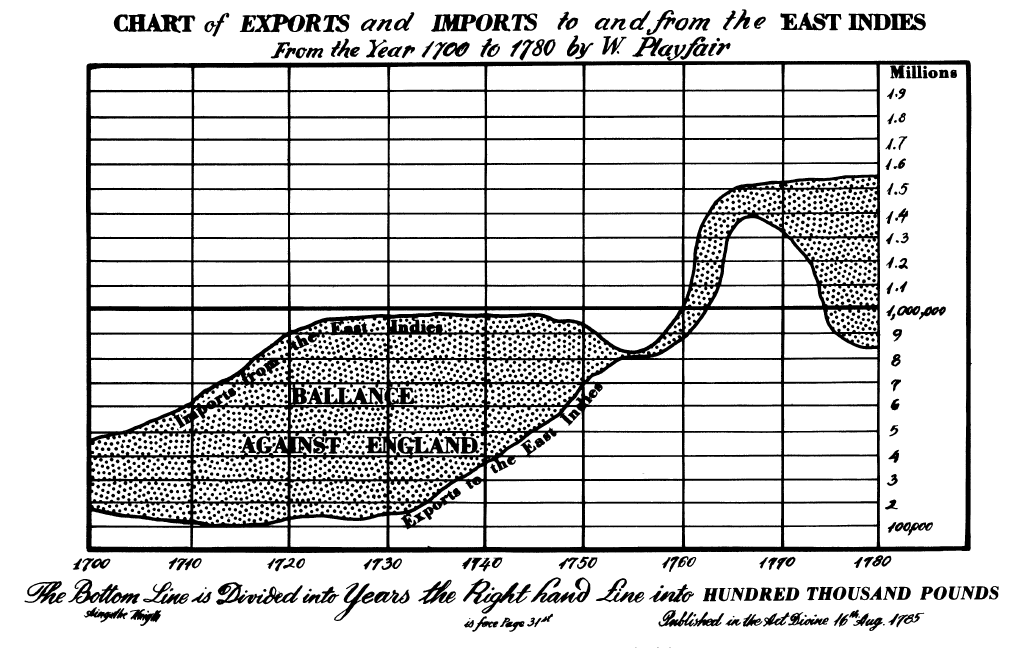
\includegraphics[width=.9\linewidth]{playfair_east_indies_gross}
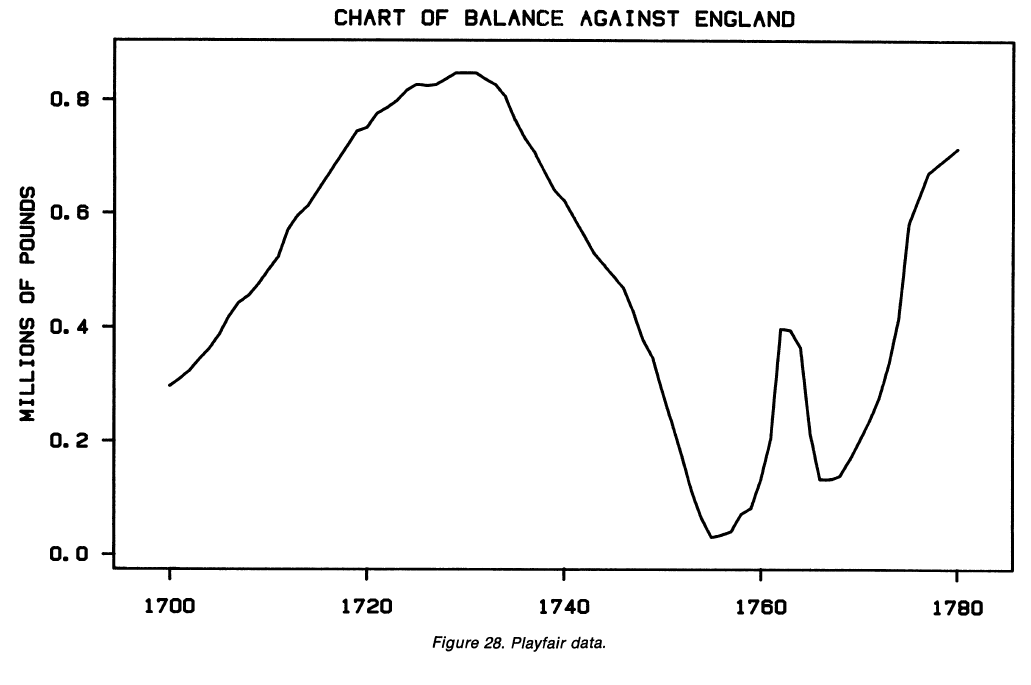
\includegraphics[width=.8\linewidth, height=.4\linewidth]{playfair_differenz_cleveland}
\caption{\label{playfair}
Playfair's chart from the Commercial and Political Atlas, 1786 (above). The sketch below shows  the difference between the lines for export and import - the steep rise in the difference around 1760  comes as a surprise to many onlookers.  }
\end{figure}


This phenomenon  is known and widely discussed in statistical graphics literature \citep{wainer:2000, robbins:2005}. It  is due to our  tendency to assess distance between curves as the minimal (orthogonal) distance rather than the  vertical distance -- see sketch \ref{fig:linewidth}.


In the perception literature, this phenomenon is known as part of a group of geometrical optical misperceptions of a context-sensitive nature classified as M\"uller-Lyer illusions \citep{day:1991}. Interestingly, there seems to be a general agreement that this illusion exists, but a quantification of it is curiously absent from the literature. 




%Figure \ref{sine-illusion} shows a screen shot of applet displaying the sine illusion. The sine illusion is closely related to the line width phenomenon -- the line segments in the are of the steepest slope of the sine curve appear to be the shortest: ``The illusion is explained in terms of a perceptual compromise between the vertical extent and the greater overall dimensions of the section at the turn of the sine-wave figure and is thereby held to be the same in principle as the M\"uller-Lyer illusion." \citep{day:1991}.
%M Bach's applet \citep{bach} gives the option to compensate the line length manually for its perceived shortcoming. The amount of compensation chosen turns out to be highly dependent on both the length of the vertical line segments and the amplitude of the sine function. The amplitude directly affects the slope -- the steeper  the slope the more compensation is necessary, see section \ref{distortion}  for a more detailed discussion and some results from a user study.
%
%
%\begin{figure}
%\centering 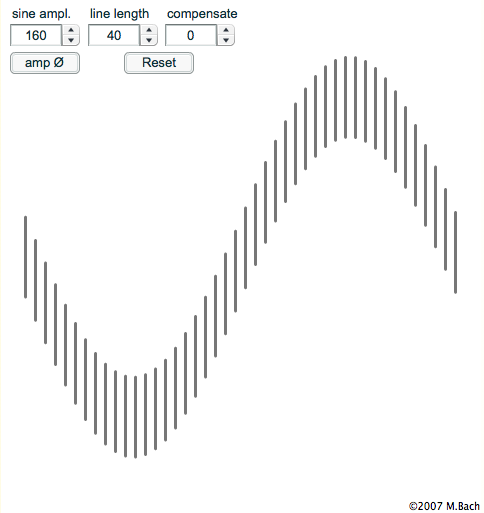
\includegraphics[width=.75\linewidth]{sine-illusion}
%\caption{Screenshot of an applet by M Bach \citep{bach} showing an example of a sine illusion. The applet is giving the possibility for compensating the line lengths in the regions with the highest slope. }
%\label{sine-illusion}
%\end{figure}




\subsection{Parallel Sets}


Parallel Sets have been introduced by R Kosara \citep{kosara:2006} as one way to visualize categorical data within the framework of parallel coordinate plots. Since initial publication, they have spread into mass media outlets: see %e.g.% 
the article on decision making and risk assessment in the BBC \citep{bbc:2009}.  While retaining the independent dimensionality that is a hallmark of parallel coordinates, Parallel Sets introduces the frequency scale that is a feature of other categorical displays such as mosaic plots \citep{kosara:2006}. Initially frequency of categories in a dimension were displayed as boxes; the latest version of Parallel Sets reduces the category placeholders to simple lines \citep{parsetredesign}. There have also been examples of reimplementation in languages other than Java \citep{davies}.  The implementation of Parallel Sets-style displays in this paper retain the original box placeholders and do not enforce a tree hierarchy via color grouping. See section Implementation for details.


\begin{figure}[hbtp]
\centering
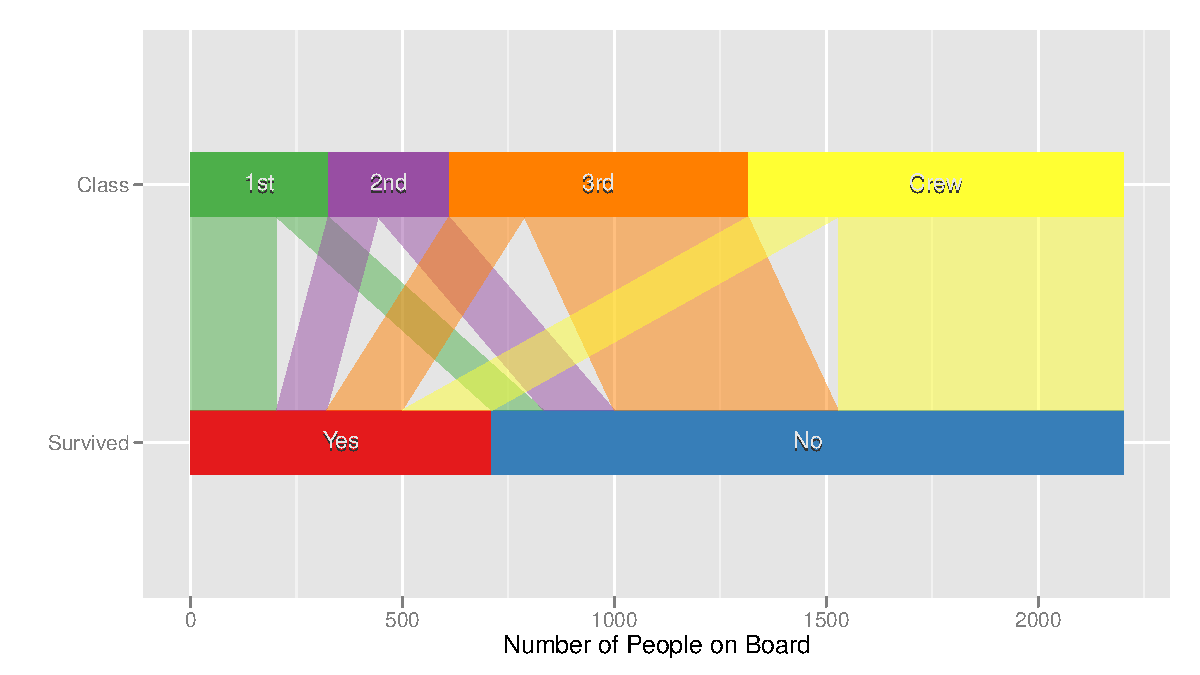
\includegraphics[width=.9\linewidth]{images/parset-titanic}
\caption{\label{question1a} Parallel sets plot showing the relationship between survival of the sinking of the HMS Titanic and class membership. }
\end{figure}

Figure \ref{question1a} gives an example for a parallel sets plot of Survival on board the HMS Titanic  \citep{dawson:1995} and its relationship to passenger status and crew membership -- this information is combined in the variable 'Class'.
 The top bar in figure \ref{question1a} shows the Class variable. Passengers are further divided into first, second or third class. The bottom bar shows survival  as yes and no. Between the bars lines are drawn to visualize the relationship between class membership and  survival. Based on the proportion of survivor and non survivors these bands are drawn from each class, and their (horizontal) width is proportional to the number of people they represent. 
%XXX PS and line-width illusion
This definition makes parallel sets susceptible to the line width illusion. When we, for example, try to order passenger class and crew membership according to their respective numbers of survivors, we need to evaluate the width of the bands between upper and lower bars in figure \ref{question1a}.
The  perceived width of the lines between the variables in figure \ref{question1a} would  lead us to assume that 1st class passengers had the highest number of survivors, followed by 3rd class passengers and about even numbers of survivors in the 2nd class  and  the crew. However, the  actual numbers are:
%
\begin{center}
\begin{tabular}{rrrrr}
& Crew & 1st & 2nd & 3rd \\ \hline
Survivors & 212 & 203 & 118 & 178\\
Non-Survivors & 673 & 122 & 167 &  528  
\end{tabular}
\end{center}
This identifies an order of crew, first class, third class, followed by second class as correct. We will discuss the origin and effects that determine the strength of the line width illusion in the next section.

The plot in figure \ref{question1a} was created using an implementation of parallel sets written for the {\tt R} environment, found in the package {\tt ggparallel} (see section Implementation). A major distinction from the most recent {\tt ParSets v2.1} Java application is the choice to remain faithful to the structure of parallel sets proposed by Kosara in \citep{kosara:2006} and display frequency of each category as scaled boxes. Maintaining visual emphasis on the marginal probabilities of categories within a single dimension \citep{parsetredesign} reduces the impact of the line-width illusion for cognizant users.

\subsection{Strength of the line width illusion}\label{distortion}

%The difference between perceived and actual line width 
The line width illusion in the parallel sets is brought on by a strong preference of evaluating the width of lines orthogonal to their slopes as opposed to horizontally (see sketch \ref{fig:linewidth}), as would be needed for a correct assessment.
Orthogonal $w_o$ and horizontal $w_h$ line widths are related -- the orthogonal line width depends on the angle (or slope) of the line:
\begin{equation}\label{adjust}
w_o = w_h \sin \theta,
\end{equation}
where $\theta$ is the angle of the line with respect to the horizontal line.

\begin{figure}[htbp]
\begin{center}
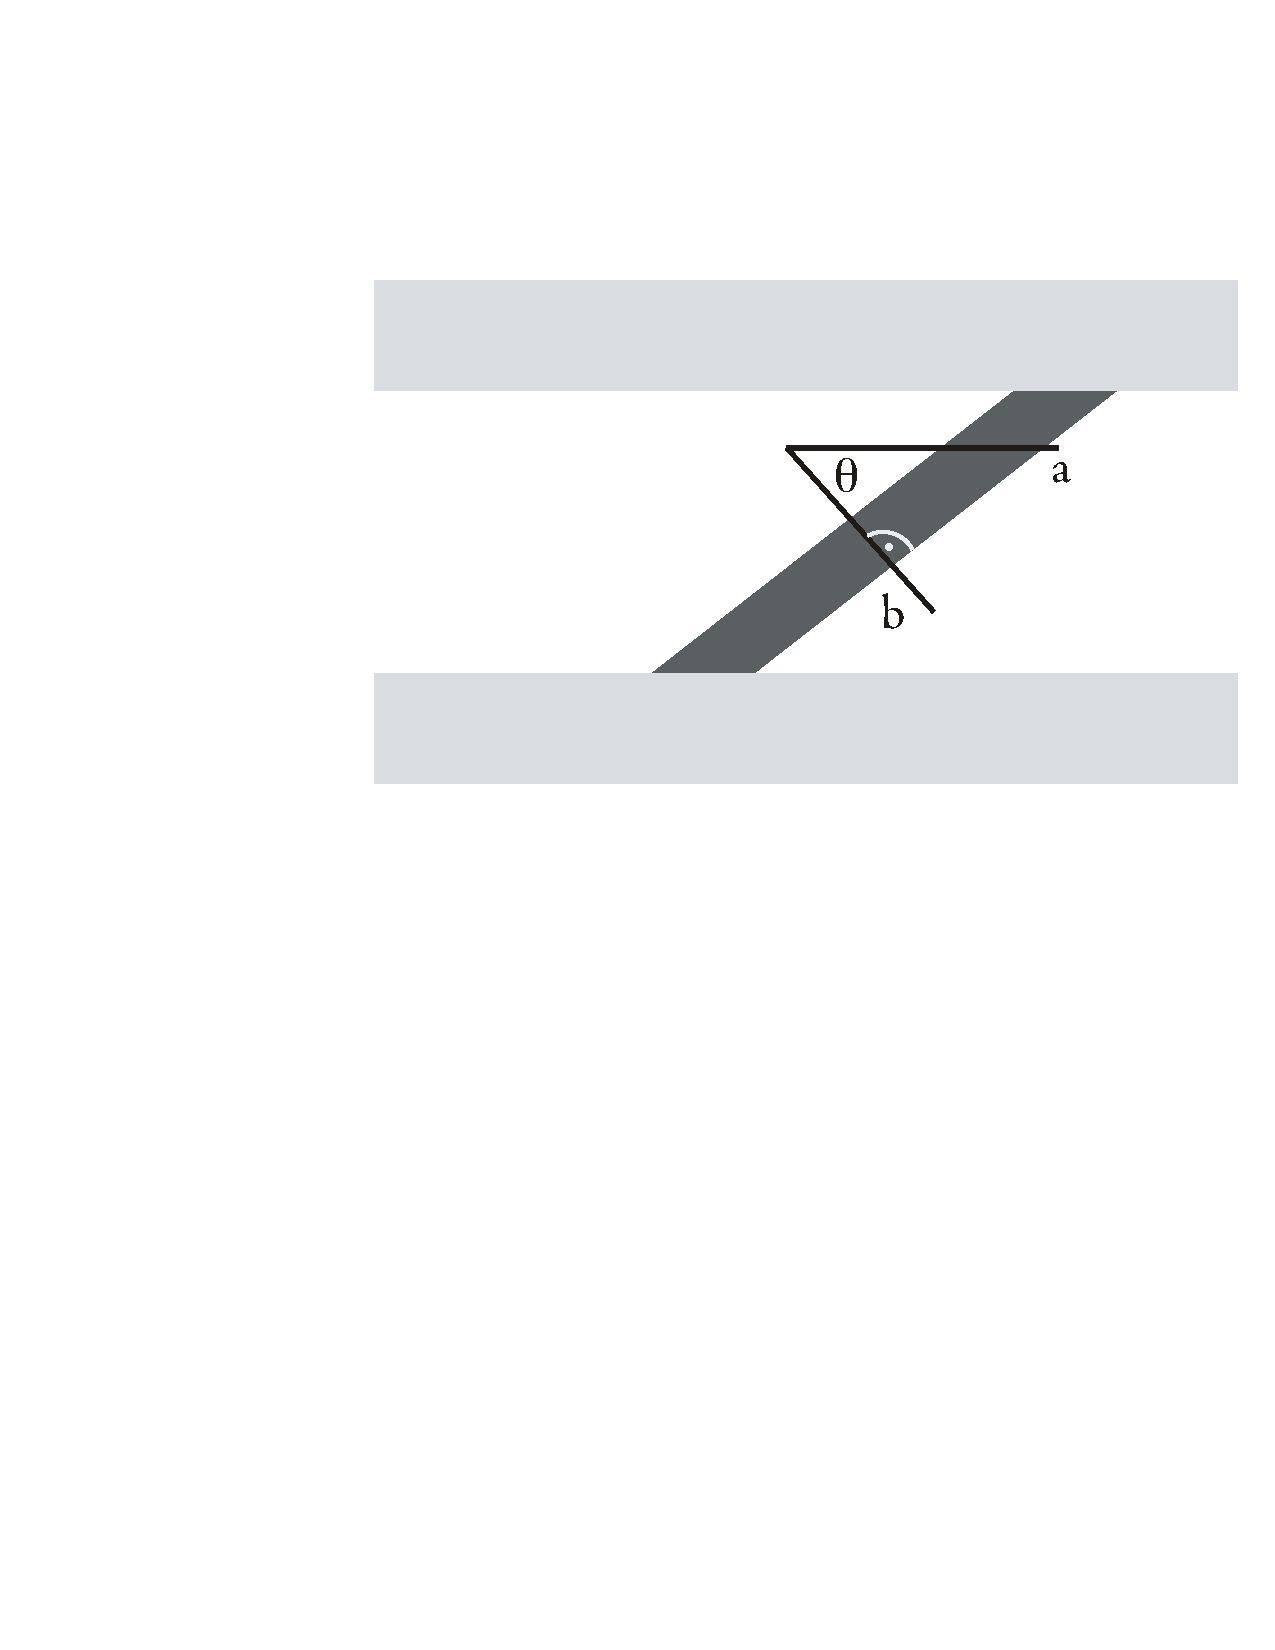
\includegraphics[width=0.6\linewidth]{images/linewidth}
\end{center}
\caption{\label{fig:linewidth}Sketch of line width assessments: (a) is showing  horizontal width, (b) shows  width orthogonal to the slope. From the survey results in section \ref{results} we can see that  observers associate line width more with  orthogonal width (b) than horizontal width (a).}
\end{figure}



%XXX aspect ratio


\begin{figure*}[htbp]
\begin{center}
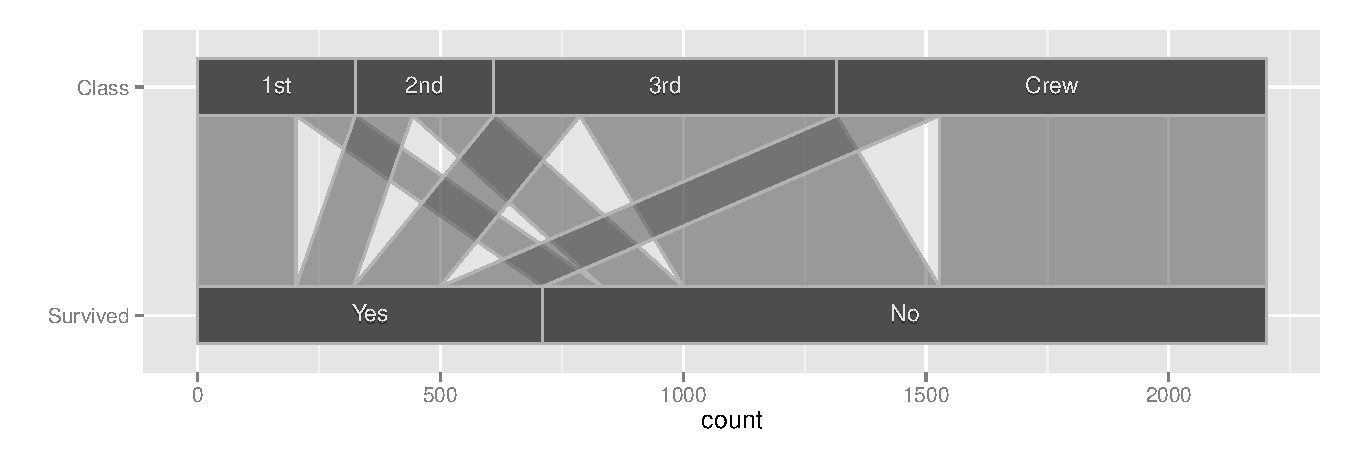
\includegraphics[height=1.5in]{images/aspect31-titanic.pdf}
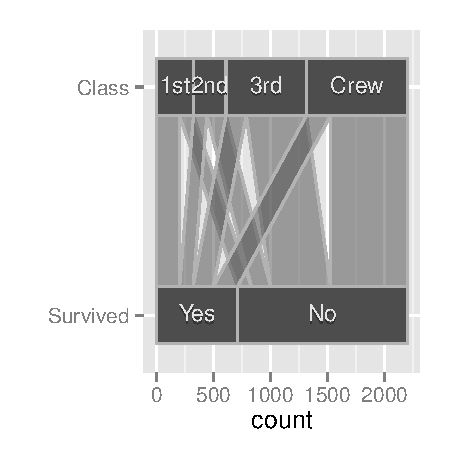
\includegraphics[height=1.5in]{images/aspect33-titanic.pdf}
\end{center}
\caption{\label{fig:aspect}Parallel sets plots of survival on the Titanic by class. Different aspect ratios  seemingly change the (orthogonal) line width, compare e.g. number of survivors in 3rd class and in the crew. }
\end{figure*}

The perceived slope of a line very much depends on the aspect ratio of the corresponding plot -- changing the height to width ratio of a display  will change our perception of the corresponding line widths, if they are not adjusted for the slope \cite{cleveland:1984}. This finding is not new, but its strength on our perception is surprising, as can be seen in the example of  figure \ref{fig:aspect}.  Again, survival and class membership on the Titanic is shown; the same parallel sets plot is shown twice in this figure, but with very different aspect ratios: in the  plot on the left the number of surviving 3rd class passengers seems to be about twice as big as the number of survivors among crew members, whereas in the plot on the right the lines have about equal (orthogonal) width. Obviously, this is not due to a change in numbers, nor a change in the way the plot is rendered. Our (intuitive) evaluation of the situation does change, though, and as designers of good graphics we have to accommodate for that the best we can. Reordering categories, as well as controlling the aspect ratio to avoid huge differences in the slope of lines helps reduce the potential of drawing wrong conclusions from these plot, but none of these measures is enough to avoid all perceptual pitfalls due to the line width illusion.








%
%\begin{figure}[hbtp]
%\begin{center}
%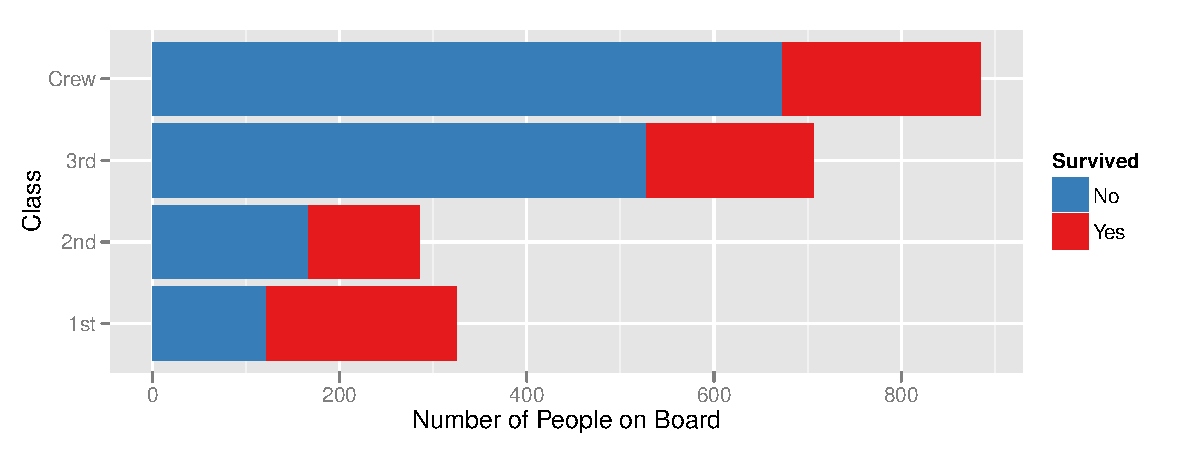
\includegraphics[width=.8\linewidth]{images/bar1-titanic}
%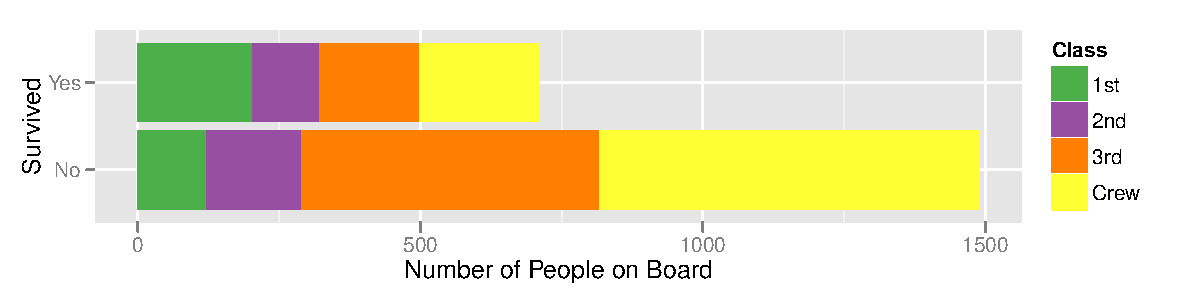
\includegraphics[width=.8\linewidth]{images/bar2-titanic}
%\end{center}
%\caption{\label{question1b} Barcharts showing Survival by Class for the Titanic Data.}
%\end{figure}



%In a preliminary survey participants were asked to order class  levels according to the number of survivors (from highest to lowest) based on  either the parallel sets plot of figure \ref{question1a} or the set of two barcharts in figure \ref{question1b} showing the same data.  
%
%% latex table generated in R 2.15.0 by xtable 1.7-0 package
%% Sat May 12 20:04:08 2012
%\begin{table}[ht]
%\begin{center}
%\begin{tabular}{rrrl}
%  \hline
% & barcharts & parallel sets & Correct \\ 
%  \hline
% 1st, 3rd, Crew,  2nd & 0 & 8 &  \\ 
%  1st, 2nd, Crew, 3rd & 0 & 4 &  \\ 
% 1st, Crew, 3rd, 2nd & 3 & 1 &  \\ 
%  Crew, 1st, 3rd, 2nd & 7 & 0 & * \\ 
%  Crew, 2nd, 3rd, 1st & 1 & 0 &  \\ 
%  Crew, 3rd, 2nd, 1st & 1 & 0 &  \\ 
%   \hline
%(all) & 12 & 13 &  \\ 
%   \hline
%\end{tabular}
%\caption{Overview of survey results: 7 out of 12 participants facing the barchart picked the correct order of `Crew, 1st, 3rd, 2nd' (highest number of survivors to lowest). None of the 13 participants evaluating the parallel set plot picked the correct result. }
%\label{tab:results}
%\end{center}
%\end{table}
%
%
%%  , , qid = 2
%%
%%                                              plottype
%%response                                       bar circos hammock
%%  1243                                           1      0       0
%%  2134                                           0      0       1
%%  3124                                           1      0       1
%%  4123                                          10      0      11
%%
%%, , qid = 3
%%
%%                                              plottype
%%response                                       bar circos hammock
%%  1342                                           1      0       1
%%  1432                                          10      0      11
%


% needed in second column of first page if using \IEEEpubid
%\IEEEpubidadjcol
\subsection{Hammock Plots}
%XXX Description of hammock plots and example

Hammock plots, introduced by M Schonlau in \citep{schonlau:2003}, provide an alternative to parallel sets that is adjusted for the line width illusion. This is done by  adjusting the --horizontal-- line width by  a factor of $\sin \theta$, as discussed in equation (\ref{adjust}). This adjustment makes the perceived --orthogonal-- line width to be proportional to the number of observations it represents. 
 Figure \ref{hammock} shows an example of a four dimensional hammock plot of the Titanic data. From top to bottom Class, Gender, Survival, and again Class are shown. 
\begin{figure}
%cols <- c(brewer.pal(name="Blues", 6)[-c(1,2)], rev(brewer.pal(name="Oranges", 3)[-1]), rev(brewer.pal(name="Greens",3)[-1]))
%ggparallel(names(titanic)[c(1,4,2,1)], order=c(0,1,1,0), method="hammock", ratio=.25, text.angle=0, titanic, weight="Freq") +
%  scale_fill_manual(values=cols, guide="none") +
%  scale_colour_manual(values=cols, guide="none") + coord_flip() 
%ggsave("hammock-titanic.pdf", width=6, height=8)
\centering
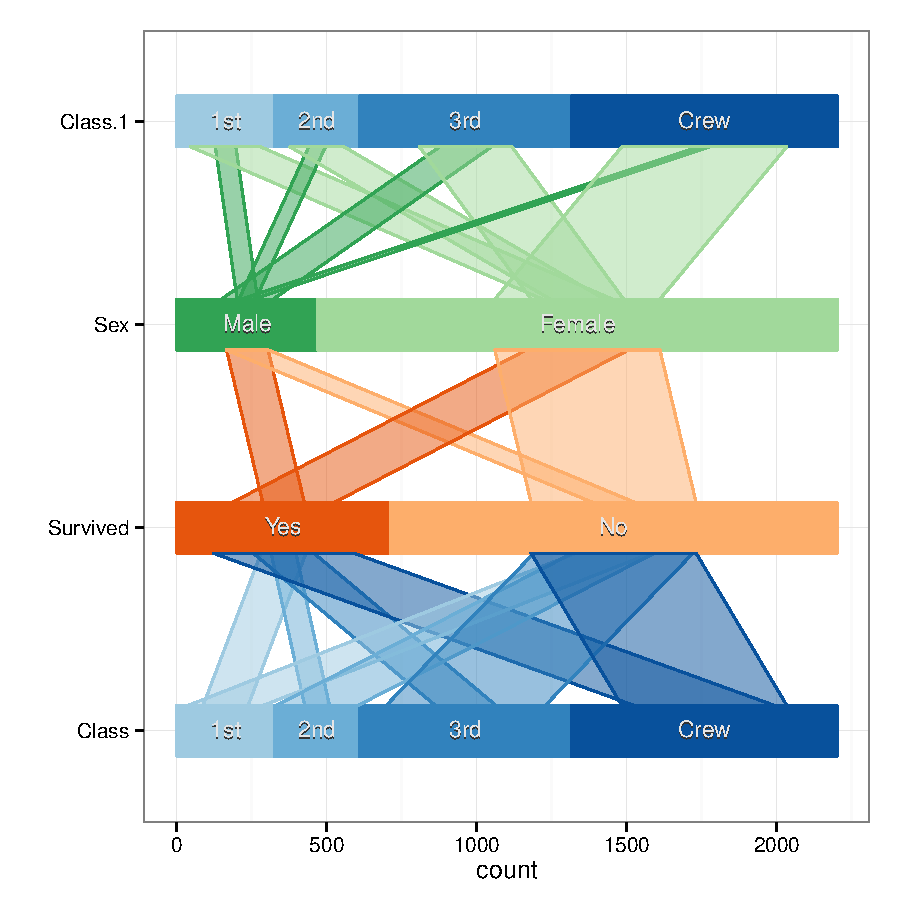
\includegraphics[width=\linewidth]{hammock-titanic}
\caption{\label{hammock} Hammock plot of the relationship between Class and Survival on the Titanic. }
\end{figure}

Similar to the parallel sets plot, the bars are divided according to class membership numbers.  Lines connect categories between neighboring bars, orthogonal line widths are representing the number of individuals in each combination. Unlike the parallel sets, the lines start from the middle of the bin and connect to the middle of the other variable's bins. 
%Line widths are adjusted in such a way, that the orthogonal width (see sketch \ref{fig:linewidth}) represents numbers.

Here, we see that barely any women were in the crew, while male crew members make up the second largest contingent overall. Overall a few more men survived than women, proportionally the situation is much different -- a much higher percentage of women survived than men. We also see, that more first class passengers survived than not, while second class passengers survival chances were about fifty-fifty. For third class passengers and crew members fewer members did  survive than not. 

As the adjustment of line widths is made with respect to the angle $\theta$, which itself depends on the aspect ratio of a plot, we need complete control over these properties of the plotting device when constructing Hammock plots  -- in our implementation (see below for details) we have dealt with this issue by fixing the aspect ratio. This is problematic in some situations, where the rendering has to be done without knowledge of the plotting device. 

Another problem that arises in evaluating hammock plots is that if an observer focuses on horizontal line width  the plots suffer from a {\it reverse line width illusion}:  judging the number of survivors by class in figure \ref{hammock} based on horizontal line width  results in an ordering of (largest to smallest) Crew, 3rd, 1st, and 2nd - which is not correct either. Using horizontal width is inviting, since the lines are centered around the middle of a level, facilitating this  comparison. 

In this paper, we propose a new approach to visualizing relationships between categorical variables in a parallel coordinate plot setting, called the {\it common angle} display. 


\section{ Common Angle Plots}
\subsection{Construction}


\begin{figure}[htbp] %  figure placement: here, top, bottom, or page
%ggparallel(names(titanic)[c(1,4,2,1)], order=c(0,1,1,0), titanic, weight="Freq", text.angle=0) + 
%  scale_fill_manual(values=cols, guide="none") +
%  scale_colour_manual(values=cols, guide="none") + coord_flip() 
%ggsave("ca-titanic.pdf", width=6, height=6)
   \centering
   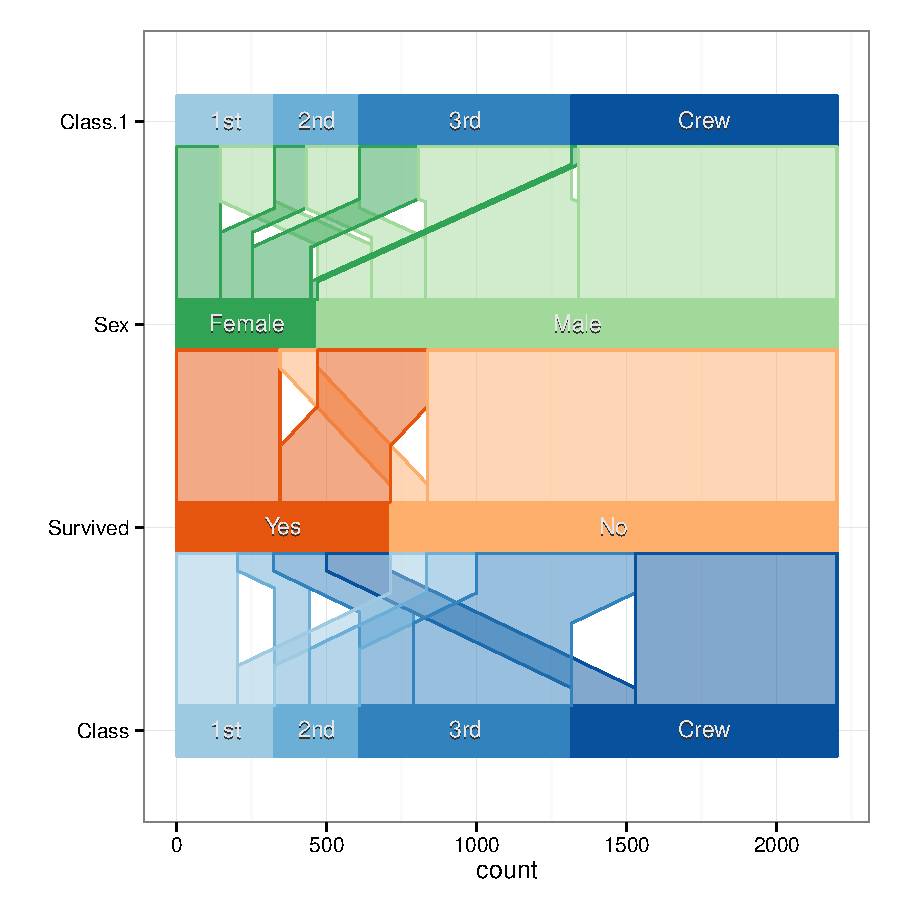
\includegraphics[width=\linewidth]{ca-titanic} 
   \caption{ \label{fig:ca-titanic} Common Angle plot of the Titanic data. }
  \end{figure}

Figure \ref{fig:ca-titanic} shows a common angle plot of the same data as the hammock plot.

As in the previously discussed display types ribbons are drawn between categories with widths  that are proportional to  the number of records they represent.

In order to ensure that  widths of all bands are  comparable without any distortion, their slopes  are artificially made the same in the following manner: 
assuming a vertical display as shown in figure \ref{fig:ca-titanic}, we modify  the connecting bands between  categories from a straight band  to a combination of a vertical  segment, a  segment under a pre-specified angle $\theta$, followed by another vertical  segment.  
The pre-specified angle $\theta$ (between the line and the vertical band) is given as --at most-- the angle of the longest connecting line between two categories of neighboring variables. 
This makes the width of ribbons  comparable without being affected by the distortion, as all ribbons are sharing at least one segment under the same angle. 

\subsection{Origins}
Historically, the common angle diagram has its roots in Sankey diagrams \citep{sankey:1898}. Sankey diagrams have their origin and main use of application in the area of industrial engineering. They are often used to show flows,  particularly, in the framework of energy consumption and losses within systems.
One of the most famous charts that can be classified as a Sankey diagram is Minard's map of Napoleon's march on Moscow \citep{minard:1812}. This map  shows the size of the army as a flow chart from West to East and the subsequent retreat. Usually, Sankey diagrams do not show a geographic co-variate, though. Modern uses of Sankey diagrams are discussed in  detail in \citep{schmidt:2008};  they can also be found in charts designed by Jen Christiansen, such as in \cite{jen3} and \cite{jen2}.

%XXX http://www.jenchristiansen.com/ Jen Christiansen 
%http://jenchristiansen.com/?p=20
%Scientific American references 
%
%Sankey diagrams William O'Brien 'Preliminary Investigation of the use of Sankey diagrams ...'

\subsection{Extension: Hammock-adjusted common angle plots}
As a logical next step in making ribbons comparable across all their parts and multiple variables, we can additionally adjust sloped parts of the ribbons using the hammock-adjustment described above. This leads to a representation as shown in figure \ref{adj.angle}. Note that ribbons no longer are required to fill the marginal bars. This choice was made to reduce the amount of overplotting resulting from the increase in width of the lines under an angle. The hammock adjustment results in re-introducing the aspect ratio as a crucial quantity. 
\begin{figure}[hbtp]
%ggparallel(names(titanic)[c(1,4,2,1)], order=c(0,1,1,0), method='adj.angle', text.angle=0, weight="Freq", titanic, ratio=0.035) + 
%  scale_fill_manual(values=cols, guide="none") +
%  scale_colour_manual(values=cols, guide="none") + coord_flip() 
%ggsave("adj-angle.pdf", width=6, height=6)
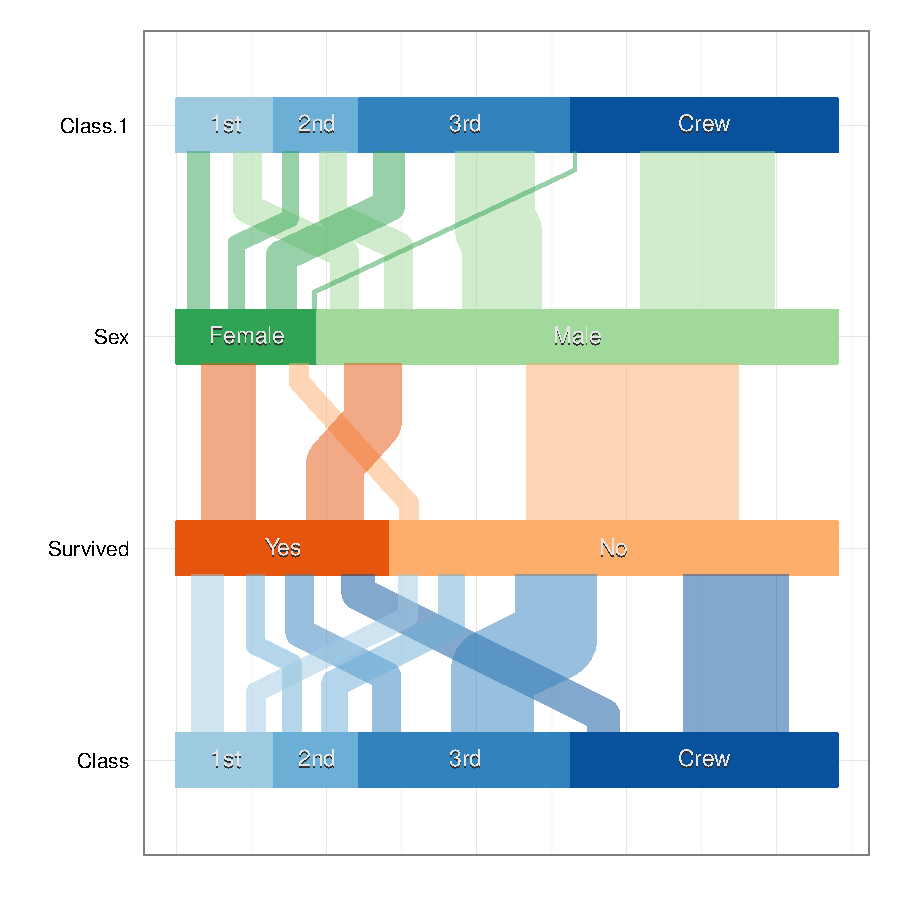
\includegraphics[width=\linewidth]{adj-angle}
\caption{\label{adj.angle} Adjusted common angle plot of the Titanic data.}
\end{figure}

\section{Evaluation}
\subsection{Survey Design}
% description of general design
To determine the effectiveness of the common angle display, we conducted a user experiment in form of a survey asking participants to provide responses regarding the structure in two data sets with predominantly categorical variables.

 All individuals were presented with the same six questions, in two blocks of three questions each. The first block of questions investigated structures in the Titanic data set, including a follow-up of the survival-class ordering issue discussed earlier. Participants were exposed to one of the three types of displays discussed: a parallel sets plot, the Hammock plot of figure \ref{hammock}, or the common angle plot of  figure \ref{fig:ca-titanic}.
 
The second block  of questions regarded gene-pathway relationships in a dataset constructed from the UCSC Genome Browser \cite{ucsc:2002} for humane genome assembly. Ribbon widths here indicate the number of genes on a  chromosome that are active in a particular pathway. The pathways we focus on here, are involved in caffeine metabolism (hsa00232),  steroid biosynthesis (hsa00100), and hsa00982, which is involved with drug metabolism via the cytochrome P450 superfamily.  One important question when dealing with drug development are interactions with other drugs. Those interactions are more likely to happen when pathways use similar locations, e.g. gene CYP1A2 is involved in both  caffeine metabolism and the drug pathway -- clomipramine (an antidepressant) and caffeine both may act as a substrate. Chromosomes give a --very rough-- approximation to location. Connections between chromosomes and pathways are therefore interesting, when they show involvement of chromosomes in several pathways.
 
%% Marie, I'm not quite sure what  clomipramine has to do with either durgs or caffeine - or is clomipramine a drug that uses hsa00982? If so, we might need an additional sentence here.
 
Participants were asked a second set of three questions (see appendix \ref{app2} for details) on this data set, but they were exposed to a  type of display different from the type accompanying questions from block 1.
  
This resulted in six different survey administrations: 

{
\scalebox{0.9}{
\begin{tabular}{rrrrrrr}
Block 1 & PS & CA & Ham & PS & CA & PS \\ 
 Block 2 & CA & PS & PS & Ham & Ham & CA \\ \hline
\#responses &  9 &  8 &  9 &  7 & 11 & 11 \\ 
\end{tabular}}}

%% however the type of chart provided as reference for answering questions varied randomly among the types described previously. 
%%
%%In the survey, participants were first asked three questions regarding the titanic dataset, three questions regarding the gene dataset,  then two questions soliciting feedback regarding plot types, allowing for free response.

\noindent
This design allows us to compare designs across different questions and data sets, while at the same time allowing to adjust for individuals' different skill sets. 
For the analysis, we first fit two linear mixed effects models, $M1$ and $M2$ -- the first one gives a general overview of comparing the designs, the second one further highlights the performance of the designs in each question.
We will then proceed to investigate some of the results in more detail.



%See appendix for details regarding the survey demographics, and data.

%XXX discussion of datasets
%XXX biological findings - pathways - what are the new findings?
%One application using biochemical pathway data is visualization of screening for drug interaction. Setting one bar to classify by pathways and a second bar to classify by physical location (e.g. chromosome), the ribbon widths indicate the number of genes on a particular chromosome that are active in a pathway. A chromosome with ribbons connecting to multiple pathways are a physical target for drugs that possibly affect both paths. In Figure XXX the bottom bar shows two pathways: hsa00232, which is involved in caffeine metabolism, and hsa00982, which is involved with drug metabolism via the cytochrome P450 superfamily. The top bar classifies by chromosome location. Gene CYP1A2 is involved in both pathways - clomipramine (an antidepressant) and caffeine both may act as a substrate.



\subsection{Results and Analysis}\label{results}
\subsubsection{Mixed effects models}
Answers for each question on the survey were assessed for correctness, giving us a binary variable of 1s and 0s, which we used to investigate performance of different designs. 

In a first model, $M1$, we are only interested in the overall difference in performance between designs. We can express this as a model of the form
\begin{equation}\label{model1}[M1]
\qquad\qquad y_i = \mu + d_{j(i)} + u_{k(i)} + \varepsilon_i \qquad\qquad
\end{equation}
where $y_i$ is the $i$th response, for $i = 1, ..., n$. $d_{j(i)}$ is the parameter measuring the effect of design $j$ ($j = C, H, P$ for \underline{C}ommon Angle, \underline{H}ammock plot, and \underline{P}arallel sets plot), $u_{k(i)}$ is the effect of participant's $k$ individual skills in evaluating these plots, $k \in \{1, ..., XXX\}$. The assumption is that skills are independent and normally distributed with an expected value of zero and a variance of $\sigma_u^2$.
$\varepsilon_i$ is, similarly to a regular linear model, assumed to be independently distributed according to a normal distribution with mean of zero and variance $\sigma^2$.

Table \ref{coef1} gives an overview of the model coefficients and their estimates. The effect of the common angle design is used as a baseline, i.e all the effects shown are differences with respect to the performance of common angle plots. Both Hammock plots and Parallel sets plot have negative effects on the correctness of the response. This indicates a significantly worse performance of these designs than under the common angle design.

Table \ref{raw} shows percentages of correctness for each design and each question. Bold numbers indicate significantly different (worse) performance of a design compared to the common angle design. Note that question $A2$ overall had the worst performance, parallel sets  exhibit significantly worse performance in four out of the six questions, Hammock plots are inferior to the common angle plot in two out the six questions. Note that in the last question Hammock plots have the best performance -- but this is does not  constitute a significant difference to the performance of the common angle design.
Also note, that the table shows raw percentages, i.e. these performance rates are not adjusted for skills of individuals. 

%xtable(summary(m1)@coefs)
% latex table generated in R 2.15.1 by xtable 1.7-0 package
% Fri Oct 12 09:08:11 2012
\begin{table}[ht]
\begin{center}
\begin{tabular}{lrrrrl}
  \hline
 & Estimate & Std. Error & z value & Pr($>$$|$z$|$) & \\ 
  \hline
$\mu$ & 1.79 & 0.25 & 7.30 & 0.00 & ***\\ [5pt]
  $d_C$& 0.00 & -- & -- & -- \\ 
  $d_H$ & -0.81 & 0.35 & -2.36 & 0.02 & * \\ 
  $d_P$ & -1.48 & 0.30 & -4.96 & 0.00 & ***\\ 
   \hline
\multicolumn{5}{l}{Signif. codes:  0 ?***? 0.001 ?**? 0.01 ?*? 0.05 ?.? 0.1 ? ? 1 }
\end{tabular}
\end{center}
\caption{\label{coef1} Model fit for $M1$ measuring correctness of answers in the survey. The common angle design is used as baseline -- both Hammock plots and, to a larger degree, Parallel sets, show a significantly worse performance.}
\end{table}


%xtable(round(acast(survey, qu~design, fun=mean, value.var="correct")*100,3), digits=1)
% latex table generated in R 2.15.1 by xtable 1.7-0 package
% Fri Oct 12 11:21:19 2012
\begin{table}[ht]
\begin{center}
\begin{tabular}{rrrr}
  \hline
 & common & hammock & parallel \\ 
  \hline
A1 & 86.0 & 74.1 & 81.5 \\ 
  A2 & 63.2 & {\bf 11.1} & {\bf 7.4} \\ 
  A3 & 73.7 & {\bf 22.2} & {\bf 18.5} \\ 
  B1 & 94.1 & 83.3 & 82.2 \\ 
  B2 & 76.5 & 68.8 & {\bf 6.7} \\ 
  B3 & 76.5 & 87.5 & {\bf 53.3} \\ 
   \hline
\end{tabular}
\end{center}
\caption{\label{raw} Raw percentages of correctness of responses for each question and design. Bold numbers indicate significant difference from common angle performances,}
\end{table}

Model $M2$ extends the first model by including both  effects for individual questions and the interaction effects with each design in the following form:
\begin{equation}\label{model2}[M2]
\quad y_i = \mu + d_{j(i)}  + q_{q(i)} + p_{j(i),q(i)} + u_{k(i)} + \varepsilon_i \quad
\end{equation}
Here, $q$ indicates the effects on performance for  each question, where $q(i)$ describes one of the questions $\{A1, A2, A3, B1, B2, B3\}$. $p$ is the parameter for the interaction effect of design and question, its index is a tuple consisting of a combination of a question and design. 

Figure \ref{fitted.m2} gives an overview of the goodness of fit of model $M2$ -- histograms of fitted values are drawn facetted by levels of the dependent variable. For correct responses fitted values are highly skewed to the left,  while most values are above 0.5. For wrong answers we see a symmetric, if not quite as clear-cut picture: fitted values are skewed right. 
Overall, Model $M2$ is a significant improvement over model $M1$ (a corresponding log-likelihood ratio test is significant at a level of $<\!\!\!< 10^{-8}$).
Table \ref{model2} shows an overview of the  parameters and their estimates for model $M2$. After adjusting for individuals' skills Parallel sets perform significantly worse than common angle plots in three of the six questions. 

\begin{figure}
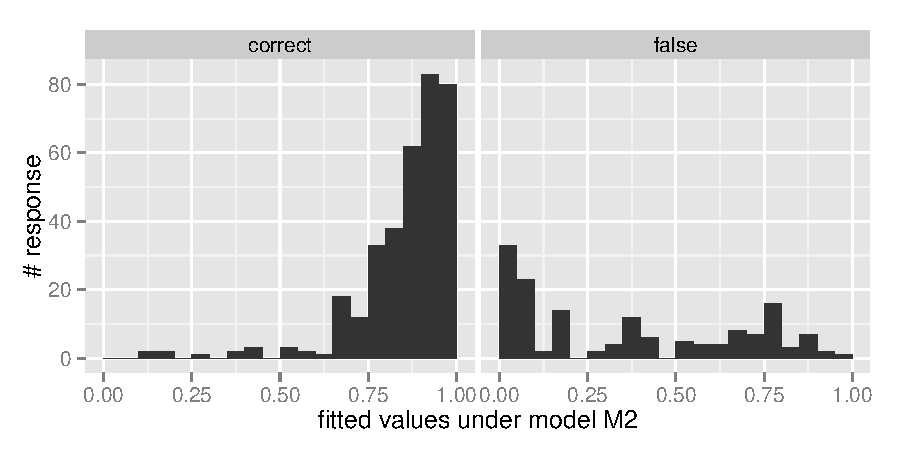
\includegraphics[width=\linewidth]{fitted-m2}
\caption{\label{fitted.m2} Histograms of fitted values under model $M2$, facetted by actual performance of participants. On the left, correct responses are shown. The histogram of fitted values is skewed to the right, with most values above 0.5. The histogram on the right corresponds to wrong answers. There are fewer wrong answers, and they tend to have low fitted values, but there are more false positives among them than false negatives for correct answers. }
\end{figure}

In the next section we will investigate the results from the survey in further detail for some questions, and highlight the link to the line width illusion and its inverse.
% xtable(summary(m4)@coefs)
% latex table generated in R 2.15.1 by xtable 1.7-0 package
% Fri Oct 12 09:12:32 2012
\begin{table}[ht]
\begin{center}
\begin{tabular}{rrrrrl}
  \hline
 & Estimate & Std. Error & z value & Pr($>$$|$z$|$) & \\ 
  \hline
$\mu$ & 2.58 & 0.56 & 4.58 & 0.00  & ***\\ [5pt]
Design\\
  $d_C$ & 0.00 & -- & -- & -- \\ 
  $d_H$ & -1.32 & 0.86 & -1.53 & 0.13 \\ 
  $d_P$ & -0.62 & 0.71 & -0.87 & 0.38 \\ [5pt]
Questions\\
  $q_{A1}$ & 0.00 & -- & -- & -- \\ 
  $q_{A2}$  & -1.75 & 0.71 & -2.46 & 0.01 &* \\ 
  $q_{A3}$  & -1.05 & 0.75 & -1.41 & 0.16 \\ 
  $q_{B1}$  & 1.43 & 1.07 & 1.33 & 0.18 \\ 
  $q_{B2}$  & -0.88 & 0.97 & -0.91 & 0.36 \\ 
  $q_{B3}$  & -0.88 & 0.97 & -0.91 & 0.36 \\ [5pt]
Interaction \\
$p_{H, A2}$ & -2.05 & 1.50 & -1.37 & 0.17 \\ 
$p_{P,A2}$ & -3.48 & 1.22 & -2.86 & 0.00 &**\\ 
$p_{H,A3}$ & -1.81 & 1.26 & -1.43 & 0.15 \\ 
$p_{P,A3}$ & -2.92 & 1.02 & -2.86 & 0.00 &**\\ 
$p_{H,B1}$ & -0.61 & 1.39 & -0.44 & 0.66 \\ 
$p_{P,B1}$ & -1.28 & 1.33 & -0.97 & 0.33 \\ 
$p_{H,B2}$ & 0.66 & 1.37 & 0.48 & 0.63 \\ 
$p_{P,B2}$ & -4.40 & 1.74 & -2.53 & 0.01 &*\\ 
$p_{H,B3}$ & 2.09 & 1.50 & 1.39 & 0.16 \\ 
$p_{P,B3}$ & -0.81 & 1.29 & -0.63 & 0.53 \\ 
   \hline
\multicolumn{5}{l}{Signif. codes:  0 ?***? 0.001 ?**? 0.01 ?*? 0.05 ?.? 0.1 ? ? 1 }
\end{tabular}
\end{center}
\caption{\label{model2} Model fit for $M2$ measuring correctness of answers in the survey, detailing performance of designs on each question. All design comparisons are with respect to the common angle design.}
\end{table}


%%%%%%%%%%%%%%
% results from preliminary survey
%Table \ref{tab:results} shows an overview of the results: 7 out of 12 participants evaluating the barcharts identified the correct order, whereas none of the 13 participants evaluating the parallel sets plot did (a Mantel-Haenszel test yields a $p$-value of 0.015, which is indicative of a significant difference between the proportions of correct answers.) The most prominent ordering for the parallel sets plot 
%put 'Crew' into third spot, while leaving the order of the other class levels unchanged. 212 members of the crew survived, while only 178 passengers of the third class did. 


%%%%%%%%%%%%%%

\subsubsection{Evidence for line width illusions}

Question $A2$ asked participants to order  class levels  according to the number of survivors, fewest to highest. There are 4! = 24 distinct orderings of the levels, corresponding to all permutations of length 4. Some orderings are closer to one another than other orderings. The Cayley distance defines a way to quantify the distance between  each pair of permutations; the Cayley distance is defined as the minimal number of transpositions, i.e. swaps of two elements,  necessary to transform one permutation into the other.
We can make use of this distance to define a graph on the space of all permutations: let all permutations be nodes of the graph; for each two permutations with a Cayley distance of one, we add an edge to this graphs. This results in a regular graph of degree six, i.e. each  node is connected to six other nodes in the graph. The Cayley distance between any two nodes is then given as the length of the shortest path between the nodes through the graph.
Figure \ref{cubes} shows an overview of the permutation space together with an overview of the survey results. Each permutation is represent by one dot. 

% - each ordering is represented by one dot. 
%XXX Discuss Caley distance: minimal number of transpositions necessary to move from one ordering to the other.
%Orderings that with a Caley distance of one, i.e.  orderings that ate only one swap of levels apart, are connected by a line, yielding a regular graph of degree 6, i.e.  each node connects to  six other nodes. 
The colored dots on top of the graph correspond to the responses from the survey - the size of the dots is proportional to the number of observers choosing this particular ordering. It becomes obvious from the three graphs in figure \ref{cubes} that
the answers to different designs occupy quite different regions, while answers based  on the same design are quite close --  usually separated by only one edge. 

The correct ordering, as well as the orderings assuming the line width illusion and its reverse are marked with symbols. Answers for the common angle design are centered around the correct answer, while responses to parallel sets are cluster around the response corresponding to the line width illusion. Due to the small number of responses to the hammock design a clear clustering of the answers is not recognizable, but the answer for the inverse line width illusion is among the responses. Table \ref{a2} gives an overview of all responses to question $A.2$. 

\begin{table}[ht]
\begin{center}
\begin{tabular}{rrrrl}
Order  & \rotatebox{90}{Common Angles}
& \rotatebox{90}{Hammock Plots}
& \rotatebox{90}{Parallel Sets} &\\
  \hline
  Crew, 1st, 3rd, 2nd &  &  2 &  \\ 
  2nd, 1st, 3rd, Crew &  &  2 &  & inverse illusion \\ 
   Crew, 3rd, 1st, 2nd &  &  1 &  1 \\ 
  2nd, 3rd, 1st, Crew & 2 & 3 & 1 \\ 
  2nd, 3rd, Crew, 1st & 12 &  1 &  2 & correct\\ 
  Crew, 3rd, 2nd, 1st &  2 &  &  \\ 
  3rd, 2nd, Crew, 1st &  1 &  &  \\ 
  1st, 2nd, 3rd, Crew &  1 &  &  2 \\ 
  1st, 3rd, Crew, 2nd &  1 &  &  3 \\ 
  Crew, 2nd, 3rd, 1st &  &  & 11 &  line width illusion\\  
  1st, 3rd, 2nd, Crew &  &  &  2 \\ 
  2nd, Crew, 3rd, 1st &  &  &  5 \\ 
   \hline
  Total & 19 &  9 & 27 \\ 
   \hline
\end{tabular}
\end{center}
\caption{\label{a2} Responses to question $A.2$: order levels of Class by the number of survivors (smallest to largest). }
\end{table}

%
Common angle displays show the best performance in terms of correctness (63.2\% on 19 responses), compared to a correctness of 7.4\% for parallel sets plots on 27 responses, indicating a significantly better performance of common angle plots at a level of 0.00022, based on a Mantel-Haenszel test (the difference in performance to Hammock plots is also significant at a level of 0.01162; but there is no significant difference in correctness between Hammock plots and parallel sets.).
While the intuitive assessment of line widths by their width orthogonal to slope is well known, it is surprising to see its strength: in this particular setting, it is strong enough to `shrink' the horizontally widest line for 11 out of 27 participants by at least  44\%, from 212 to below 118, and a further 5 participants perceived the shrinking to below 178, which constitutes a distortion of at least 16\%.

\begin{figure*}
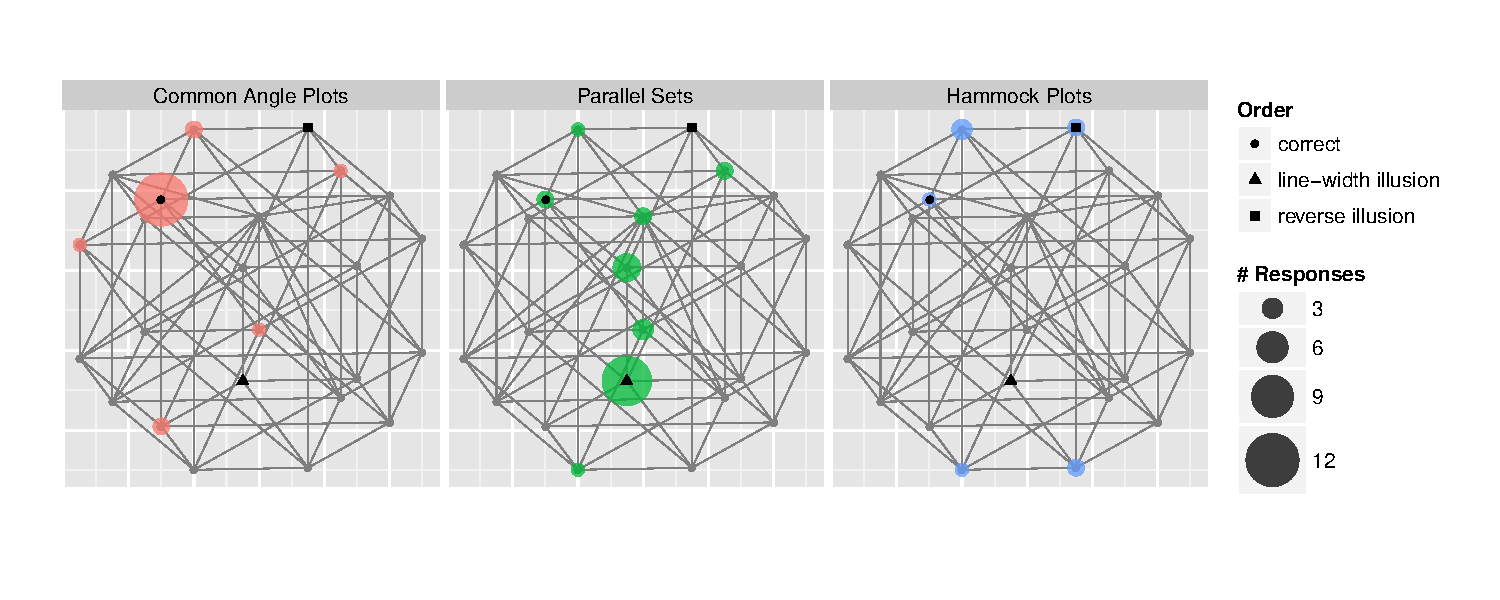
\includegraphics[width=\linewidth]{cubes}
\caption{Answers to question A.2 -- each node corresponds to a single ordering of the levels in variable 'Class'. Lines are drawn between orderings that are only one swap of levels apart. The colored dots show responses from the survey, their sizes depend on the number of responses for each ordering. }
\label{cubes}
\end{figure*}

Responses to question A.3 exhibit a similar pattern, see table \ref{a3}.

\begin{table}[ht]
\begin{center}
\begin{tabular}{rrrrl}
Order &  \rotatebox{90}{Common Angles}
& \rotatebox{90}{Hammock Plots}
& \rotatebox{90}{Parallel Sets} &\\
  \hline
c, b, a &  &  2 &  \\
a, b, c &  1 &  5 &  & inverse illusion\\ 
a, c, b & 14 &  2 &  5 & correct\\ 
b, c, a &  2 &  &  2 \\ 
c, a, b &  2 &  & 15 & line width illusion\\ 
b, a, c &  &  &  5 \\ 
 \hline
  Total & 19 &  9 & 27 \\ 
   \hline
\end{tabular}
\end{center}
\caption{\label{a3}Responses to question A.3: order combinations from smallest to largest, where 'a' is first class female, 'b' are male survivors, and 'c' are crew survivors. }
\end{table}



\begin{table}[ht]
\begin{center}
\begin{tabular}{clrrrl}
  Qu & Design & \rotatebox{90}{Correct} & \rotatebox{90}{Incorrect} & \rotatebox{90}{No Answer}   & Reason\\ \hline
  \hline
1 & common &   16 &  0 &   1 \\ 
   & hammock &   15 &  0 &   1 \\ 
 & parallel &   7 &   8 &   0 & line width illusion\\ \hline
2 & common &  16 &   0 &   1 \\ 
& hammock &   9 &   7 &   0 & inverse illusion\\ 
& parallel &  15 &   0 &   0 \\ \hline
3& common &  16 &   0 &   1 \\ 
& hammock &  16 &   0 &   0 \\ 
& parallel &  15 &   0 &   0 \\ 
   \hline
\end{tabular}
\end{center}
\caption{\label{tab:b1}Responses to question B.1}
\end{table}

Table \ref{tab:b1} shows a summary to the  three questions of $B.1$ with possible answers ``agree", ``disagree", and ``don't know".
The first two questions are  examples, where the line width illusion, and its reverse will lead to answers that differ from the correct answer. Parallel sets plots are susceptible to the line width illusion, while hammock plots suffer from the reverse. The data shows that in about 50\% of the responses we can see this difference. 8 out of 15 answers for the parallel sets plots in question 1 deviate from the correct answer, and 7 out of 16 responses corresponding to hammock plots in question 2 show the wrong answer.



%\begin{figure*}[htbp] %  figure placement: here, top, bottom, or page
%   \centering
%   \includegraphics[width=\linewidth]{caffeine_drug} 
%   \caption{Common gene activity for caffeine and drug metabolism}
%   \label{fig:caffeine}
%\end{figure*}


\section{Implementation}

All  of the discussed variants of parallel coordinate plots for categorical data are implemented as part of the package {\tt ggparallel} based on the {\tt ggplot2} \cite{ggplot2} plotting framework in the software {\tt R} 2.15.1 \citep{R}. The  {\tt ggparallel} package is freely available from CRAN (\url{http://www.r-project.org/}).
The colors for the plots have been chosen using color schemes from the ColorBrewer project  \cite{colorbrewer} , as implemented in the R package {\tt RColorBrewer}  \cite{RColorBrewer} .


\section{Conclusion}
%The conclusion goes here. The conclusion goes here.The conclusion goes here.The conclusion goes here.The conclusion goes here.The conclusion goes here.The conclusion goes here.The conclusion goes here.The conclusion goes here.The conclusion goes here.The conclusion goes here.The conclusion goes here.The conclusion goes here.The conclusion goes here.The conclusion goes here.The conclusion goes here.The conclusion goes here.The conclusion goes here.The conclusion goes here.The conclusion goes here. The conclusion goes here.The conclusion goes here.The conclusion goes here.The conclusion goes here.





% if have a single appendix:
%\appendix[Proof of the Zonklar Equations]
% or
%\appendix  % for no appendix heading
% do not use \section anymore after \appendix, only \section*
% is possibly needed

% use appendices with more than one appendix
% then use \section to start each appendix
% you must declare a \section before using any
% \subsection or using \label (\appendices by itself
% starts a section numbered zero.)
%

%
\appendix
%\subsection*{Demographics of the pre-cursory survey I}\label{app1}
%33 students, staff and faculty from Iowa State University participated in the survey investigating the strength of the perceptual line width distortion. The Qualtrics system \cite{} was used to create the survey and all students, staff and faculty from programs in Statistics, Bioinformatics and Computational Biology and Human Computer Interaction were invited to participate by email. No personally identifiable information was collected, nor was any compensation offered. Participants used their own personal computing devices to access the survey. A majority of participants used WoW64 (Windows 32-bit or Windows 64-bit), with the next most common operating system Intel Mac OS X10.6.8 (Snow Leopard). The preferred choice of browser was  Chrome, followed by Firefox. For two participants, the Qualtrics survey software was unable to capture operating system or browser information.
%
%One question in this survey asked participants to rank the number of survivors in the titanic dataset by class. The results are summarized in table  \ref{tab:results} .


%No participants chose to do so using internet explorer. 

% ## operating system
% summary(df2$Q2_3_TEXT)
% #                      Intel Mac OS X 10_6_8 Intel Mac OS X 10_7_3   Intel Mac OS X 10.6          Linux x86_64 
% #                    2                     7                     4                     1                     3 
% #               rv:6.0                Ubuntu                 WOW64 
% #                    1                     1                    14 
% 
% ## browser info
% ### NOTE: I discovered after the survey went out that IE renders the html code for the training data poorly
% summary(df2$Q2_1_TEXT)
% #         Chrome Firefox  Safari 
% #      2      16      10       5 

% In contrast to that, a second question asking participants to order class levels according to survival {\it rates} of members did not yield any indication that parallel sets were performing less efficiently than barcharts; 11 out of 12 (barcharts) and 12 out of 13 (parallel sets) participants were able to answer this question correctly. The answer was also based on either figure \ref{question1a} or \ref{question1b}. While the line width illusion is present, its effect for this instance is not strong enough to have an impact on the order of the results.



\subsection*{Survey }\label{app2}
All students, staff and faculty from Iowa State University programs in Statistics, Bioinformatics and Computational Biology and Human Computer Interaction were invited to participate by email. 93 individuals accessed the survey, with 47 individuals submitting responses for all questions. As in the first survey, participants used their own personal computing devices to access the survey, which was created using Qualtrics Labs, Inc software. No personally identifiable information was collected, nor was any compensation offered. At the survey start, participants were presented a brief tutorial regarding the different plot types.  \\

\noindent The questions pertaining to the titanic dataset were: \\ \\
\begin{itemize}
\item[A1.]\emph{Agree, Disagree or Don't Know/Can't Determine with the following statements:}
\begin{itemize}
\item There were an approximately equal number of Male and Female Survivors
\item The group with largest number of travelers was Female Survivors
\item There were more Male Non-Survivors than number of males in First AND Second Class Combined
\end{itemize}

\item[A2.]\emph{Order the categories of Class by number Survived, fewest to most.} 
\begin{itemize}
\item 1st
\item 2nd 
\item 3rd
\item Crew
\end{itemize}

\item[A3.]\emph{Order the following groups by number, fewest to most}
\begin{itemize}
\item 1st Class female passengers
\item Male Survivors
\item Crew Survivors
\end{itemize}
\end{itemize}


\noindent \\  The questions pertaining to the gene dataset were: 


\begin{itemize}
\item[B1.]\emph{Agree, Disagree or Don't Know/Can't Determine with the following statements:}
\begin{itemize}
\item There are about the same number of genes in the group "steroid biosynthesis:chromosome 1" as in the group "caffeine metabolism: chromosome 8"
\item The group with the greatest number of genes is "drug metabolism:chromosome 4"
\item there are more genes involved in the group "drug metabolism: chromosome 1" than all genes involved in the caffeine metabolism pathway
\end{itemize}

\item[B2.]\emph{Order the following chromosomes by number of genes involved in steroid biosynthesis pathway, fewest to most.}
\begin{itemize}
\item chromosome 1
\item chromosome 4
\item chromosome 8 
\item chromosome X
\end{itemize}

\item[B3.]\emph{Order the following chromosomes by number of genes involved, fewest to most.}
\begin{itemize}
\item steroid biosynthesis :: chromosome X
\item steroid biosynthesis :: chromosome 4
\item drug metabolism :: chromosome X
\end{itemize} 
\end{itemize} 

\noindent \\Participants were randomly assigned to one of six blocks, each of approximately equal size. While individuals in all blocks were presented with the same questions and datasets in the order shown above, each block was presented with a unique ordering of only two of the plot types (e.g parallel sets and hammock plot; common angles and parallel sets, etc) to use as reference when respon. This study design structure was imposed, in part,  to encourage participation by reducing the amount of time for survey completion. Completion of all survey questions was anticipated to take 10 - 15 minutes.

\subsection*{Data and preprocessing}
Data for questions A1, A2 and A3 in survey 2 were previously published in: \citep{dawson:1995}.

Data for questions B1, B2 and B3 in survey 2 was obtained using the UCSC Genome Browser \cite{ucsc:2002} for humane genome assembly (hg18, May2006). The data was subsetted for genes involved in pathways hsaXXX (drug metabolism), hsaXXX (caffeine metabolism), and hsaXXX (steroid biosynthesis). From this data, genes active on selected chromosomes were displayed in plots.

All data manipulation was performed  using software {\tt R} 2.15.1 \citep{R} with Bioconductor package KEGG.db \cite{kegg}
%
%\subsection*{Discussion of Sine Illusion}
%Using the notation given in the applet, we assume a value $s$ for the sine amplitude, $\ell$ for the vertical length of line segments, and $\ell_c$ for the amount of compensation. 
%The sine curve is then given by function $f$, written as 
%\[
%f(x) = s/2 \sin(x)
%\]
%for $x$ in $[-\pi, \pi]$. The slope of the sine curve is the steepest in its reflection point at $x=0$. We can calculate the slope as $f^\prime(x) = s/2 \cos(x)$, which in $x=0$ yields a slope of $s/2$.
%
%The physical dimensions of the applet are 500 pixels by 500 pixels, corresponding to an extent in the $x$ axis of $2 \pi$ and a maximum amplitude and line lengths of 250 in the $y$ axis. This results in an aspect ratio of $250 : (2\pi)$.
%For the physical angle $\theta$ of the slope with respect to the horizontal axis we get
%\[
%\tan \theta =  s/2 \cdot 2\pi/250 = s\pi/250
%\]
%Adding a compensation of $\ell_c$ to the length of line segments is supposed to make the orthogonal width of the region of the steepest slope appear as wide as the vertical length in the turning point. Since the slope in the turning point is zero, the extent of the width is unchanged and is therefore equal to $\ell$. 
%We therefore get for an `optimal' compensation as
%\[
%\ell \stackrel{!}{=} \cos \theta \cdot \left( \ell + \ell_c \right),
%\]
%yielding 
%\[
%\ell_c = \left(1 - \cos \theta\right)/\cos \theta \ \  \ell.
%\]
%theta <- function(s) atan(s*pi/250)
%compensate <- function(theta) (1-cos(theta))/cos(theta)



% use section* for acknowledgement
\ifCLASSOPTIONcompsoc
  % The Computer Society usually uses the plural form
  \section*{Acknowledgments}
\else
  % regular IEEE prefers the singular form
  \section*{Acknowledgment}
\fi


The survey for this study was carried out with approval from  IRB-ID 12-204.


% Can use something like this to put references on a page
% by themselves when using endfloat and the captionsoff option.
\ifCLASSOPTIONcaptionsoff
  \newpage
\fi



% trigger a \newpage just before the given reference
% number - used to balance the columns on the last page
% adjust value as needed - may need to be readjusted if
% the document is modified later
%\IEEEtriggeratref{8}
% The "triggered" command can be changed if desired:
%\IEEEtriggercmd{\enlargethispage{-5in}}

% references section

% can use a bibliography generated by BibTeX as a .bbl file
% BibTeX documentation can be easily obtained at:
% http://www.ctan.org/tex-archive/biblio/bibtex/contrib/doc/
% The IEEEtran BibTeX style support page is at:
% http://www.michaelshell.org/tex/ieeetran/bibtex/
\bibliographystyle{IEEEtran}
% argument is your BibTeX string definitions and bibliography database(s)
\bibliography{references}
%
% <OR> manually copy in the resultant .bbl file
% set second argument of \begin to the number of references
% (used to reserve space for the reference number labels box)
%\begin{thebibliography}{1}
%
%\bibitem{IEEEhowto:kopka}
%%This is an example of a book reference
%H. Kopka and P.W. Daly, \emph{A Guide to {\LaTeX}}, third ed. Harlow, U.K.: Addison-Wesley, 1999.
%
%
%%This is an example of a Transactions article reference
%%D.S. Coming and O.G. Staadt, "Velocity-Aligned Discrete Oriented Polytopes for Dynamic Collision Detection," IEEE Trans. Visualization and Computer Graphics, vol.?14,? no.?1,? pp. 1-12,? Jan/Feb? 2008, doi:10.1109/TVCG.2007.70405.
%
%%This is an example of a article from a conference proceeding
%%H. Goto, Y. Hasegawa, and M. Tanaka, "Efficient Scheduling Focusing on the Duality of MPL Representation," Proc. IEEE Symp. Computational Intelligence in Scheduling (SCIS '07), pp. 57-64, Apr. 2007, doi:10.1109/SCIS.2007.367670.
%
%%This is an example of a PrePrint reference
%%J.M.P. Martinez, R.B. Llavori, M.J.A. Cabo, and T.B. Pedersen, "Integrating Data Warehouses with Web Data: A Survey," IEEE Trans. Knowledge and Data Eng., preprint, 21 Dec. 2007, doi:10.1109/TKDE.2007.190746.
%
%%Again, see the IEEEtrans_HOWTO.pdf for several more bibliographical examples. Also, more style examples
%%can be seen at http://www.computer.org/author/style/transref.htm
%\end{thebibliography}

% biography section
% 
% If you have an EPS/PDF photo (graphicx package needed) extra braces are
% needed around the contents of the optional argument to biography to prevent
% the LaTeX parser from getting confused when it sees the complicated
% \includegraphics command within an optional argument. (You could create
% your own custom macro containing the \includegraphics command to make things
% simpler here.)
%\begin{biography}[{\includegraphics[width=1in,height=1.25in,clip,keepaspectratio]{mshell}}]{Michael Shell}
% or if you just want to reserve a space for a photo:

\begin{IEEEbiography}{Heike Hofmann}
Biography text here.
\end{IEEEbiography}

\begin{IEEEbiography}{Marie Vendettuoli}
Biography text here.
\end{IEEEbiography}

% if you will not have a photo at all:
%\begin{IEEEbiographynophoto}{John Doe}
%Biography text here.Biography text here.Biography text here.Biography text here.Biography text here.Biography text here.Biography text here.Biography text here.Biography text here.Biography text here.Biography text here.Biography text here.Biography text here.Biography text here.Biography text here.Biography text here.Biography text here.Biography text here.Biography text here.Biography text here.Biography text here.Biography text here.Biography text here.Biography text here.Biography text here.Biography text here.Biography text here.Biography text here.Biography text here.Biography text here.Biography text here.Biography text here.
%\end{IEEEbiographynophoto}
%
%% insert where needed to balance the two columns on the last page with
%% biographies
%%\newpage
%
%\begin{IEEEbiographynophoto}{Jane Doe}
%Biography text here.Biography text here.Biography text here.Biography text here.Biography text here.Biography text here.Biography text here.Biography text here.Biography text here.Biography text here.Biography text here.Biography text here.Biography text here.Biography text here.Biography text here.Biography text here.Biography text here.Biography text here.Biography text here.Biography text here.Biography text here.Biography text here.Biography text here.Biography text here.Biography text here.Biography text here.Biography text here.Biography text here.
%\end{IEEEbiographynophoto}

% You can push biographies down or up by placing
% a \vfill before or after them. The appropriate
% use of \vfill depends on what kind of text is
% on the last page and whether or not the columns
% are being equalized.

%\vfill

% Can be used to pull up biographies so that the bottom of the last one
% is flush with the other column.
%\enlargethispage{-5in}



% that's all folks
\end{document}



